\section{What This Chapter Defines}

\subsection{From Intuition to Formalism}

The previous chapter established the \textit{problem}: classical computers are structurally blind. This chapter presents the \textit{solution}: the Thiele Machine, a computational model where structure is a first-class resource.

% =====================================================
% FIGURE: Chapter 3 Roadmap
% =====================================================
\begin{figure}[ht]
\centering
\begin{tikzpicture}[
    box/.style={draw, rounded corners, minimum width=4.6cm, minimum height=1.7cm, align=center, font=\normalsize},
    arrow/.style={->, >=stealth, thick},
    dasharrow/.style={->, >=stealth, very thick, dashed},
    scale=0.65, transform shape
, node distance=3cm]
% Main components
\node[box, fill=blue!20, align=center, text width=3.5cm, font=\normalsize] (state) at (0,0) {State Space\\$S$};
\node[box, fill=green!20, align=center, text width=3.5cm, font=\normalsize] (partition) at (4,0) {Partition Graph\\$\Pi$};
\node[box, fill=orange!20, align=center, text width=3.5cm, font=\normalsize] (axioms) at (8,0) {Axiom Set\\$A$};
\node[box, fill=red!20, align=center, text width=3.5cm, font=\normalsize] (rules) at (4,-2.5) {Transition Rules\\$R$};
\node[box, fill=purple!20, align=center, text width=3.5cm, font=\normalsize] (logic) at (8,-2.5) {Logic Engine\\$L$};

% Central element
\node[box, fill=yellow!30, minimum width=6.2cm, minimum height=2.2cm, align=center, text width=3.5cm, font=\normalsize] (mu) at (0,-2) {$\mu$-Ledger\\(Currency)};

% Arrows
\draw[arrow, shorten >=2pt, shorten <=2pt] (state) -- (partition) node[pos=0.5, font=\small, above, yshift=6pt] {decomposition};
\draw[arrow, shorten >=2pt, shorten <=2pt] (partition) -- (axioms) node[pos=0.5, font=\small, above, yshift=6pt] {constraints};
\draw[arrow, shorten >=2pt, shorten <=2pt] (rules) -- (state) node[pos=0.5, font=\small, above, yshift=6pt] {evolves};
\draw[arrow, shorten >=2pt, shorten <=2pt] (logic) -- (axioms) node[pos=0.5, font=\small, above, yshift=6pt] {verifies};
\draw[arrow, shorten >=2pt, shorten <=2pt] (rules) -- (mu) node[pos=0.5, font=\small, above, yshift=6pt] {charges};
\draw[dasharrow, shorten >=2pt, shorten <=2pt] (mu) -- (state) node[pos=0.5, font=\small, above, yshift=6pt] {bounds};

% Title
\node[above=1.0cm of partition,  font=\small, yshift=6pt] {The Thiele Machine: $T = (S, \Pi, A, R, L)$};

% Sections
\node[ below=0.3cm of state, above, font=\small, yshift=6pt] {§3.2.1};
\node[ below=0.3cm of partition, above, font=\small, yshift=6pt] {§3.2.2};
\node[ below=0.3cm of axioms, above, font=\small, yshift=6pt] {§3.2.3};
\node[ below=0.3cm of rules, above, font=\small, yshift=6pt] {§3.2.4};
\node[ below=0.3cm of logic, above, font=\small, yshift=6pt] {§3.2.5};
\node[ below=0.3cm of mu, above, font=\small, yshift=6pt] {§3.3};
\end{tikzpicture}
\caption{Chapter 3 roadmap: The five components of the Thiele Machine and their relationships. The $\mu$-ledger (center-left) is the central innovation that ``charges'' operations and ``bounds'' the state evolution.}
\label{fig:ch3_roadmap}
\end{figure}

\paragraph{Understanding Figure \ref{fig:ch3_roadmap}:}

\textbf{Five components (boxes):}
\begin{itemize}
    \item \textbf{State Space $S$ (blue):} Registers, memory, PC. What the machine remembers. §3.2.1
    \item \textbf{Partition Graph $\Pi$ (green):} State decomposition into modules. §3.2.2
    \item \textbf{Axiom Set $A$ (orange):} Logical constraints on modules. §3.2.3
    \item \textbf{Transition Rules $R$ (red):} 18-instruction ISA. §3.2.4
    \item \textbf{Logic Engine $L$ (purple):} SMT oracle for verification. §3.2.5
\end{itemize}

\textbf{Central element:} $\mu$-Ledger (yellow) - the currency tracking structural cost. §3.3

\textbf{Relationships:} State $\to$ Partition (decomposition), Partition $\to$ Axioms (constraints), Rules $\to$ State (evolves), Logic $\to$ Axioms (verifies), Rules $\to$ $\mu$ (charges), $\mu$ $\dashrightarrow$ State (bounds). The $\mu$-ledger is fed by transition rules and bounds state evolution.

\textbf{Role:} Chapter roadmap showing how formal components relate.

The model is defined formally because informal descriptions are ambiguous. A formal definition:
\begin{itemize}
    \item Eliminates ambiguity: Every term has a precise meaning
    \item Enables proof: I can mathematically prove properties
    \item Ensures implementation: The formal definition guides code
\end{itemize}

\subsection{The Five Components}

The Thiele Machine has five components:
\begin{enumerate}
    \item \textbf{State Space $S$}: What the machine "remembers"---registers, memory, partition graph
    \item \textbf{Partition Graph $\Pi$}: How the state is \textit{decomposed} into independent modules
    \item \textbf{Axiom Set $A$}: What logical constraints each module satisfies
    \item \textbf{Transition Rules $R$}: How the machine evolves---the 18-instruction ISA
    \item \textbf{Logic Engine $L$}: The oracle that verifies logical consistency
\end{enumerate}
Each component corresponds to a concrete artifact in the formal development. The state and partition graph are defined in \path{coq/kernel/VMState.v}; the instruction set and step relation are defined in \path{coq/kernel/VMStep.v}; and the logic engine is represented by certificate checkers in \path{coq/kernel/CertCheck.v}. The point of the 5-tuple is not cosmetic: it is a decomposition that forces every later proof to say which resource it uses (state, partitions, axioms, transitions, or certificates), so that any implementation layer can mirror the same structure without guessing.

\subsection{The Central Innovation: $\mu$-bits}

The key innovation is the \textit{$\mu$-bit currency}---a unit of structural information cost. Every operation that adds structural knowledge to the system charges a cost in $\mu$-bits. This cost is:
\begin{itemize}
    \item \textbf{Monotonic}: Once paid, $\mu$-bits are never refunded
    \item \textbf{Bounded}: The $\mu$-ledger lower-bounds irreversible operations
    \item \textbf{Observable}: The cost is visible in the execution trace
\end{itemize}
In the formal kernel, the ledger is the field \texttt{vm\_mu} in \texttt{VMState}, and every opcode carries an explicit \texttt{mu\_delta}. The step relation in \path{coq/kernel/VMStep.v} defines \texttt{apply\_cost} as \texttt{vm\_mu + instruction\_cost}, so the ledger increases exactly by the declared cost and never decreases. The extracted runner exports \texttt{vm\_mu} as part of its JSON snapshot, and the RTL testbench prints $\mu$ in its JSON output for partition-related traces; individual isomorphism gates then compare only the fields relevant to the trace type.

\subsection{How to Read This Chapter}

This chapter is technical and formal. It defines:
\begin{itemize}
    \item The state space and partition graph (§3.1)
    \item The instruction set (§3.4)
    \item The $\mu$-bit currency and conservation laws (§3.5--3.6)
    \item The No Free Insight theorem (§3.7)
\end{itemize}

\textbf{Key definitions to understand}:
\begin{itemize}
    \item \texttt{VMState} (the state record)
    \item \texttt{PartitionGraph} (how state is decomposed)
    \item \texttt{vm\_step} (how the machine transitions)
    \item \texttt{vm\_mu} (the $\mu$-ledger)
\end{itemize}
These names are not placeholders: they are the exact identifiers used in \path{coq/kernel/VMState.v} and \path{coq/kernel/VMStep.v}. When later chapters mention a “state” or a “step,” they mean these concrete definitions and the proofs that refer to them.

If the formalism becomes overwhelming, refer to Chapter 4 (Implementation) for concrete code examples.

\subsection{Key Concepts: Observables and Projections}

\begin{tcolorbox}[colback=green!5!white,colframe=green!75!black,title=\textbf{Observables and State Projections}]
\begin{definition}[Observable]
An \textbf{observable} is a function $\text{Obs}: S \to \mathcal{O}$ that extracts a verifiable property from state $S$. For a module with ID $\text{mid}$, the observable is:
\[
\text{Observable}(s, \text{mid}) = \begin{cases}
(\text{normalize}(\text{region}), \mu) & \text{if module exists} \\
\bot & \text{otherwise}
\end{cases}
\]
Note: Axioms are \emph{not} observable---they are internal implementation details.
\end{definition}

\begin{definition}[State Projection]
A \textbf{state projection} $\pi: S \to S'$ maps full machine state to a canonical subset used for cross-layer comparison. Different verification gates use different projections:
\begin{itemize}
    \item \textbf{Compute gate}: projects registers and memory
    \item \textbf{Partition gate}: projects canonicalized module regions
    \item \textbf{Full projection}: includes pc, $\mu$, err, regs, mem, csrs, and graph
\end{itemize}
\end{definition}
\end{tcolorbox}

\section{The Formal Model: $T = (S, \Pi, A, R, L)$}

The Thiele Machine is formally defined as a 5-tuple $T = (S, \Pi, A, R, L)$, representing a computational system that is explicitly aware of its own structural decomposition.

\subsection{State Space $S$}

The state space $S$ represents the complete instantaneous description of the machine. Unlike the flat tape of a Turing Machine, $S$ is a structured record containing multiple components.

% =====================================================
% FIGURE: VMState Record Structure
% =====================================================
\begin{figure}[ht]
\centering
\begin{tikzpicture}[scale=1.8, 
    node distance=3cm,
    field/.style={draw, minimum width=10.8cm, minimum height=1.2cm, font=\ttfamily\small, align=left},
    every node/.style={font=\normalsize}
]
% VMState box
\node[draw, very thick, minimum width=12.6cm, minimum height=10.8cm, fill=gray!5] (vmstate) at (0,0) {};
\node[above=0.3cm of vmstate.north, font=\bfseries\ttfamily, pos=0.5, font=\small, yshift=6pt] {VMState};

% Fields
\node[field, fill=green!15] (graph) at (0, 2.2) {vm\_graph : PartitionGraph};
\node[field, fill=blue!15] (csrs) at (0, 1.4) {vm\_csrs : CSRState};
\node[field, fill=blue!10] (regs) at (0, 0.6) {vm\_regs : list nat (32)};
\node[field, fill=blue!10] (mem) at (0, -0.2) {vm\_mem : list nat (256)};
\node[field, fill=orange!15] (pc) at (0, -1.0) {vm\_pc : nat};
\node[field, fill=yellow!30] (mu) at (0, -1.8) {vm\_mu : nat};
\node[field, fill=red!15] (err) at (0, -2.6) {vm\_err : bool};

% Annotations
\node[label, right=1.0cm of graph, font=\small, xshift=10pt] {$\leftarrow$ \textit{Partition structure}};
\node[label, right=1.0cm of csrs, font=\small, xshift=10pt] {$\leftarrow$ \textit{Control registers}};
\node[label, right=1.0cm of regs, font=\small, xshift=10pt] {$\leftarrow$ \textit{Register file}};
\node[label, right=1.0cm of mem, font=\small, xshift=10pt] {$\leftarrow$ \textit{Data memory}};
\node[label, right=1.0cm of pc, font=\small, xshift=10pt] {$\leftarrow$ \textit{Program counter}};
\node[label, right=1.0cm of mu, font=\small, xshift=10pt] {$\leftarrow$ \textbf{$\mu$-ledger (key!)}};
\node[label, right=1.0cm of err, font=\small, xshift=10pt] {$\leftarrow$ \textit{Error flag}};

% Highlight mu
\draw[ultra very thick, red!70!black] ($(mu.north west)+(-0.1,0.1)$) rectangle ($(mu.south east)+(0.1,-0.1)$);
\end{tikzpicture}
\caption{The \texttt{VMState} record structure. The $\mu$-ledger (\texttt{vm\_mu}) is highlighted as the central innovation---a monotonic counter tracking cumulative structural cost.}
\label{fig:vmstate_record}
\end{figure}

\paragraph{Understanding Figure \ref{fig:vmstate_record}:}

\textbf{Seven fields:}
\begin{itemize}
    \item \textbf{vm\_graph (green):} PartitionGraph - state decomposition structure
    \item \textbf{vm\_csrs (blue):} CSRState - control/status registers
    \item \textbf{vm\_regs (blue):} list nat (32) - register file
    \item \textbf{vm\_mem (blue):} list nat (256) - data memory
    \item \textbf{vm\_pc (orange):} nat - program counter
    \item \textbf{vm\_mu (yellow, very thick red border):} nat - \textbf{$\mu$-ledger (KEY!)}
    \item \textbf{vm\_err (red):} bool - error flag
\end{itemize}

\textbf{Highlighted field:} vm\_mu with ultra-very thick red border - the central innovation. This monotonic counter tracks cumulative structural cost.

\textbf{Key insight:} Complete state snapshot in one record. Immutable in Coq (transitions create new states). vm\_mu never decreases.

\subsubsection{Formal Definition}

In the formal development, the state is defined as:

\begin{lstlisting}
Record VMState := {
  vm_graph : PartitionGraph;
  vm_csrs : CSRState;
  vm_regs : list nat;
  vm_mem : list nat;
  vm_pc : nat;
  vm_mu : nat;
  vm_err : bool
}.
\end{lstlisting}

\paragraph{Understanding the VMState Record:} This Coq \texttt{Record} defines a product type—a structure where all fields coexist simultaneously. Think of it as a snapshot of the entire machine state at a given moment. In Coq, a \texttt{Record} is syntactic sugar for an inductive type with a single constructor, making it convenient to define and access structured data.

\textbf{From First Principles:} A state machine requires complete information to determine its next state. This record provides exactly that information—nothing more, nothing less. Each field represents a distinct aspect of the computational state:
\begin{itemize}
    \item \textbf{Type Safety:} Each field has an explicit type (e.g., \texttt{nat} for natural numbers, \texttt{bool} for booleans). Coq's type system prevents misuse at compile time.
    \item \textbf{Immutability:} In Coq, values are immutable. State transitions create new \texttt{VMState} values rather than mutating existing ones, enabling equational reasoning.
    \item \textbf{Totality:} Every \texttt{VMState} must have all fields defined. There's no concept of ``null'' or ``undefined''—the state is always complete and well-formed.
\end{itemize}

Each component serves a specific purpose:
\begin{itemize}
    \item \textbf{vm\_graph}: The partition graph $\Pi$, encoding the current decomposition of the state into modules
    \item \textbf{vm\_csrs}: Control Status Registers including certification address, status flags, and error codes
    \item \textbf{vm\_regs}: A register file of 32 registers (matching RISC-V conventions)
    \item \textbf{vm\_mem}: Data memory of 256 words
    \item \textbf{vm\_pc}: The program counter
    \item \textbf{vm\_mu}: The $\mu$-ledger accumulator
    \item \textbf{vm\_err}: Error flag (latching)
\end{itemize}
The sizes are not arbitrary: \texttt{REG\_COUNT} and \texttt{MEM\_SIZE} are defined in \path{coq/kernel/VMState.v} and are mirrored in the Python and RTL layers so that indexing and wrap-around are identical. Reads and writes use modular indexing (\texttt{reg\_index} and \texttt{mem\_index}) so that any out-of-range access deterministically folds back into the fixed-width state, matching the hardware behavior where wires have fixed width.

\subsubsection{Word Representation}

The machine uses 32-bit words with explicit masking:
\begin{lstlisting}
Definition word32_mask : N := N.ones 32.
Definition word32 (x : nat) : nat :=
  N.to_nat (N.land (N.of_nat x) word32_mask).
\end{lstlisting}

\paragraph{Understanding Word Masking:} These definitions ensure fixed-width arithmetic behavior, crucial for matching hardware semantics.

\textbf{Breaking Down the Code:}
\begin{enumerate}
    \item \textbf{\texttt{N.ones 32}}: Creates a binary number with 32 consecutive 1-bits: \texttt{0xFFFFFFFF}. This is our bitmask. The \texttt{N} type represents binary natural numbers optimized for bit operations.
    
    \item \textbf{\texttt{N.of\_nat x}}: Converts from Coq's mathematical natural numbers (\texttt{nat}, defined inductively as \texttt{O | S nat}) to the binary representation (\texttt{N}). Why? Because \texttt{nat} is convenient for proofs but inefficient for computation.
    
    \item \textbf{\texttt{N.land}}: Bitwise AND operation. When we AND any number with \texttt{0xFFFFFFFF}, we keep only the lower 32 bits and discard everything above. Example: \texttt{0x1FFFFFFFF AND 0xFFFFFFFF = 0xFFFFFFFF}.
    
    \item \textbf{\texttt{N.to\_nat}}: Converts back to \texttt{nat} for use in the rest of the formal model.
\end{enumerate}

\textbf{Why This Matters:} Coq's \texttt{nat} type represents unbounded natural numbers (0, 1, 2, 3, ..., $\infty$). Real hardware uses fixed-width registers. Without explicit masking, \texttt{0xFFFFFFFF + 1} would be \texttt{0x100000000} in Coq but \texttt{0x00000000} in hardware (overflow/wraparound). By applying \texttt{word32} after every operation, we enforce hardware semantics in the mathematical model.

This ensures that all arithmetic operations properly wrap at $2^{32}$, so word-level behavior is explicit and deterministic.
In the Coq kernel, write operations (\texttt{write\_reg} and \texttt{write\_mem}) mask values through \texttt{word32}, so every stored word is explicitly truncated rather than implicitly relying on the host language. This makes the arithmetic model match the RTL and avoids ambiguities where a high-level language might use unbounded integers.

\subsection{Partition Graph $\Pi$}

The partition graph is the central innovation of the Thiele Machine. It represents the decomposition of the state into modules, with disjointness enforced by the partition operations that construct and modify those modules.

% =====================================================
% FIGURE: Partition Graph Visualization
% =====================================================
\begin{figure}[ht]
\centering
\begin{tikzpicture}[
    module/.style={draw, rounded corners, minimum width=4.0cm, minimum height=2.4cm, align=center, font=\normalsize},
    memory/.style={draw, minimum width=0.6cm, minimum height=0.6cm, font=\normalsize},
    scale=0.65, transform shape
, node distance=3cm]
% Memory addresses (background)
\foreach \i in {0,...,15} {
    \node[memory, fill=gray!20] (m\i) at (\i*0.5-4, -3) {\i};
}

% Module M1
\node[module, fill=blue!20, align=center, text width=3.5cm, font=\normalsize] (M1) at (-2.5, 0) {Module $M_1$\\ID: 0};
\draw[blue, very thick, ->, shorten >=2pt, shorten <=2pt] (M1.south) -- (-3.25, -2.7);
\draw[blue, very thick, ->, shorten >=2pt, shorten <=2pt] (M1.south) -- (-2.75, -2.7);
\foreach \i in {0,1} {
    \node[memory, fill=blue!40] at (\i*0.5-4, -3) {\i};
}

% Module M2
\node[module, fill=green!20, align=center, text width=3.5cm, font=\normalsize] (M2) at (1, 0) {Module $M_2$\\ID: 1};
\draw[green!60!black, very thick, ->, shorten >=2pt, shorten <=2pt] (M2.south) -- (0.25, -2.7);
\draw[green!60!black, very thick, ->, shorten >=2pt, shorten <=2pt] (M2.south) -- (0.75, -2.7);
\draw[green!60!black, very thick, ->, shorten >=2pt, shorten <=2pt] (M2.south) -- (1.25, -2.7);
\foreach \i in {8,9,10} {
    \node[memory, fill=green!40] at (\i*0.5-4, -3) {\i};
}

% Module M3
\node[module, fill=orange!20, align=center, text width=3.5cm, font=\normalsize] (M3) at (4.5, 0) {Module $M_3$\\ID: 2};
\draw[orange, very thick, ->, shorten >=2pt, shorten <=2pt] (M3.south) -- (3.25, -2.7);
\foreach \i in {14} {
    \node[memory, fill=orange!40] at (\i*0.5-4, -3) {\i};
}

% Partition Graph box
\node[draw, dashed, very thick, minimum width=21.6cm, minimum height=4.6cm={above:\textbf{PartitionGraph}}] at (1, 0) {};

% Next ID indicator
\node[draw, fill=purple!20, rounded corners] (nextid) at (4.5, 1.5) {\texttt{pg\_next\_id = 3}};

% Memory label
\node[below=0.5cm of m8,  font=\small, yshift=-6pt] {Memory addresses (0--15)};

% Axioms
\node[ below=0.3cm of M1, above, font=\small, yshift=6pt] {$A = \{x > 0\}$};
\node[ below=0.3cm of M2, above, font=\small, yshift=6pt] {$A = \{\}$};
\node[ below=0.3cm of M3, font=\small, yshift=-6pt] {$A = \{y \text{ prime}\}$};

% Key properties
\node[draw, fill=white, rounded corners, font=\normalsize, align=left, align=center, text width=3.5cm] at (-5.5, 0) {
    \textbf{Properties:}\\
    $\bullet$ ID monotonic\\
    $\bullet$ Regions disjoint\\
    $\bullet$ Ops preserve WF
};
\end{tikzpicture}
\caption{A partition graph with three modules. Each module ``owns'' a disjoint region of memory addresses. Module IDs are monotonically increasing (\texttt{pg\_next\_id} tracks the next available ID). Axioms are attached to each module but are not externally observable.}
\label{fig:partition_graph_viz}
\end{figure}

\paragraph{Understanding Figure \ref{fig:partition_graph_viz}:}

\textbf{Bottom:} Memory addresses 0-15 (gray squares)

\textbf{Three modules (colored boxes):}
\begin{itemize}
    \item \textbf{Module $M_1$ (blue):} ID=0, owns addresses \{0,1\} (highlighted blue)
    \item \textbf{Module $M_2$ (green):} ID=1, owns addresses \{8,9,10\} (highlighted green)
    \item \textbf{Module $M_3$ (orange):} ID=2, owns address \{14\} (highlighted orange)
\end{itemize}

\textbf{Key properties:}
\begin{itemize}
    \item \textbf{Disjoint:} No address appears in multiple modules
    \item \textbf{Monotonic IDs:} 0, 1, 2 (pg\_next\_id tracks next available)
    \item \textbf{Axioms:} Attached to each module (not shown in visual - internal)
\end{itemize}

\textbf{Dashed bounding box:} PartitionGraph container

\textbf{Role:} Shows state decomposition - each module is an independent structural unit.

\subsubsection{Formal Definition}

\begin{lstlisting}
Record PartitionGraph := {
  pg_next_id : ModuleID;
  pg_modules : list (ModuleID * ModuleState)
}.

Record ModuleState := {
  module_region : list nat;
  module_axioms : AxiomSet
}.
\end{lstlisting}

\paragraph{Understanding the Partition Graph Structure:} These two records define the core data structure for tracking decomposition.

\textbf{PartitionGraph Analysis:}
\begin{itemize}
    \item \textbf{pg\_next\_id}: Acts as a monotonic counter ensuring unique module IDs. Starting from 0, each new module increments this value. This prevents ID collisions and provides a total ordering over module creation time.
    \item \textbf{pg\_modules}: An association list (list of pairs) mapping each \texttt{ModuleID} to its \texttt{ModuleState}. Think of this as a dictionary or hash table in other languages, but implemented as an immutable list for provability.
\end{itemize}

\textbf{ModuleState Analysis:}
\begin{itemize}
    \item \textbf{module\_region}: A list of memory addresses (natural numbers) that this module "owns." These addresses are disjoint from other modules' regions—no two modules can claim the same address.
    \item \textbf{module\_axioms}: Logical constraints about the data in this region. For example, "all values are positive" or "this region stores a sorted array." These are verified by external SMT solvers.
\end{itemize}

\textbf{Design Rationale:} Why use lists instead of sets or arrays? Because Coq's list type has extensive proven libraries (\texttt{List.v}), making verification easier. The performance cost (O(n) lookup) is acceptable because the number of modules is typically small ($<$100), and this is a \emph{specification}, not an optimized implementation.

Key properties and intended semantics:
\begin{itemize}
    \item \textbf{ID Monotonicity}: Module IDs are monotonically increasing (all existing IDs are strictly less than \texttt{pg\_next\_id}). This is the invariant enforced globally.
    \item \textbf{Disjointness}: Module regions are intended to be disjoint. This is enforced by checks during operations such as \texttt{PMERGE} (which rejects overlapping regions) and \texttt{PSPLIT} (which validates disjoint partitions).
    \item \textbf{Coverage}: Partition operations ensure that a split covers the original region and that merges preserve region union. Global coverage of all machine state is not required; modules describe only the regions explicitly placed under partition structure.
\end{itemize}
The graph is therefore a compact, explicit record of \emph{what has been structurally separated so far}. Nothing in the kernel assumes a universal partition over memory; the model only tracks the modules that have been explicitly introduced by \texttt{PNEW}, \texttt{PSPLIT}, and \texttt{PMERGE}. This distinction is essential: if a region has never been partitioned, it remains “structurally opaque,” and the model refuses to grant any insight about its internal structure without paying $\mu$.

\subsubsection{Well-Formedness Invariant}

The partition graph must satisfy a well-formedness invariant focused on ID discipline:
\begin{lstlisting}
Definition well_formed_graph (g : PartitionGraph) : Prop :=
  all_ids_below g.(pg_modules) g.(pg_next_id).
\end{lstlisting}

\paragraph{Understanding Well-Formedness:} This definition establishes a crucial invariant that must hold at all times.

\textbf{Breaking It Down:}
\begin{itemize}
    \item \textbf{Prop}: In Coq, \texttt{Prop} is the universe of logical propositions. This is not a computable function returning true/false; it's a mathematical statement that is either provable or not.
    \item \textbf{all\_ids\_below}: A predicate (defined elsewhere) asserting that every \texttt{ModuleID} in the module list is strictly less than \texttt{pg\_next\_id}.
    \item \textbf{g.(field)}: Coq syntax for accessing record fields. This is notation for \texttt{pg\_modules g} and \texttt{pg\_next\_id g}.
\end{itemize}

\textbf{Why This Invariant?} It ensures that \texttt{pg\_next\_id} is always a valid "fresh" ID. When creating a new module, we can safely use \texttt{pg\_next\_id} knowing it doesn't conflict with existing IDs, then increment it. This is the standard technique for generating unique identifiers in functional programming.

\textbf{Logical Implication:} If this invariant holds, then the partition graph is internally consistent—no module has an ID greater than or equal to the next available ID. This prevents temporal paradoxes where a module appears to be created "in the future."

This invariant is proven to be preserved by all operations:
\begin{itemize}
    \item \texttt{graph\_add\_module\_preserves\_wf}
    \item \texttt{graph\_remove\_preserves\_wf}
    \item \texttt{wf\_graph\_lookup\_beyond\_next\_id}
\end{itemize}
The well-formedness invariant is deliberately minimal. It does \emph{not} require disjointness or coverage; those properties are enforced locally by the specific graph operations that need them. By keeping the invariant small (all IDs are below \texttt{pg\_next\_id}), the proofs about step semantics and extraction become simpler and do not assume extra structure that is not actually needed to execute the machine.

\subsubsection{Canonical Normalization}

Regions are stored in canonical form to ensure observational equivalence:
\begin{lstlisting}
Definition normalize_region (region : list nat) : list nat :=
  nodup Nat.eq_dec region.
\end{lstlisting}

\paragraph{Understanding Region Normalization:}
\textbf{What \texttt{nodup} Does:} This function removes duplicate elements from a list while preserving the order of first occurrence. Given \texttt{[3; 1; 4; 1; 5; 9; 3]}, it returns \texttt{[3; 1; 4; 5; 9]}.

\textbf{The \texttt{Nat.eq\_dec} Parameter:} Coq requires a decidable equality function to compare elements. \texttt{Nat.eq\_dec} is a proven decision procedure that returns either \texttt{left (a = b)} (proof of equality) or \texttt{right (a $\neq$ b)} (proof of inequality) for any natural numbers a and b. This is more powerful than a simple boolean comparison—it provides a \emph{proof witness}.

\textbf{Why Normalize?} Two lists \texttt{[1; 2; 1]} and \texttt{[2; 1]} represent the same \emph{set} of addresses. Normalization ensures a unique canonical representation, making equality checking straightforward and deterministic.

The key lemma ensures idempotence:
\begin{lstlisting}
Lemma normalize_region_idempotent : forall region,
  normalize_region (normalize_region region) = normalize_region region.
\end{lstlisting}

\paragraph{Understanding Idempotence:}
\textbf{Mathematical Definition:} A function $f$ is idempotent if $f(f(x)) = f(x)$ for all inputs $x$. Applying it multiple times has the same effect as applying it once.

\textbf{Why This Lemma Matters:} It proves that normalization is stable—once a region is normalized, it stays normalized. This is critical for:
\begin{enumerate}
    \item \textbf{Equality Checking:} We can compare normalized regions directly without worrying about further transformations.
    \item \textbf{Proof Simplification:} When reasoning about operations, we know that \texttt{normalize(normalize(r))} can be simplified to \texttt{normalize(r)}.
    \item \textbf{Canonical Forms:} Ensures every equivalence class has exactly one representative.
\end{enumerate}

This ensures that repeated normalization does not change the representation, which makes observables stable across equivalent encodings.
The point is to remove duplicate indices while preserving the original order of first occurrence. This makes region equality depend only on set content (not on multiplicity), which is crucial for observational equality: two modules that mention the same indices in different orders should be treated as equivalent once normalized.

\subsection{Axiom Set $A$}

Each module carries a set of axioms—logical constraints that the module satisfies.

\subsubsection{Representation}

Axioms are represented as strings in SMT-LIB 2.0 format:
\begin{lstlisting}
Definition VMAxiom := string.
Definition AxiomSet := list VMAxiom.
\end{lstlisting}

\paragraph{Understanding the String-Based Axiom System:}
\textbf{Type Alias Pattern:} These are type aliases (like typedef in C). \texttt{VMAxiom} is just another name for \texttt{string}, and \texttt{AxiomSet} is a list of strings. This provides semantic clarity in type signatures without changing runtime behavior.

\textbf{Why Strings Instead of Parsed ASTs?}
\begin{enumerate}
    \item \textbf{Separation of Concerns:} The Thiele Machine kernel doesn't need to understand logical formulas—it just stores and forwards them. Parsing logic belongs in the checker (Z3, CVC4), not the kernel.
    \item \textbf{Extensibility:} New logical theories can be added without modifying the kernel. Want to add non-linear arithmetic? Just write new SMT-LIB strings.
    \item \textbf{Verifiability:} The kernel's trusted computing base (TCB) is smaller because it doesn't contain a formula parser/evaluator.
    \item \textbf{Interoperability:} SMT-LIB 2.0 is an industry standard. Any compliant solver can check our axioms.
\end{enumerate}

This choice keeps the kernel agnostic to the internal structure of logical formulas. The kernel does not parse or interpret these strings; it only passes them to certified checkers (see \path{coq/kernel/CertCheck.v}) and records them as part of a module's logical commitments.

For example, an axiom asserting that a variable $x$ is non-negative might be:
\begin{lstlisting}
"(assert (>= x 0))"
\end{lstlisting}

\paragraph{Understanding SMT-LIB Axiom Syntax:}
\textbf{String Literal:} The entire axiom is a Coq string (enclosed in quotes), containing SMT-LIB syntax.

\textbf{SMT-LIB S-Expression Breakdown:}
\begin{itemize}
    \item \textbf{Parentheses}: Delimit function application (prefix notation)
    \item \textbf{assert}: SMT-LIB command to add a constraint to the solver
    \item \textbf{(>= x 0)}: The constraint formula
    \begin{itemize}
        \item \textbf{>=}: Greater-than-or-equal predicate
        \item \textbf{x}: A variable (must be declared previously)
        \item \textbf{0}: Integer literal
        \item \textbf{Reading}: "$x \geq 0$"
    \end{itemize}
\end{itemize}

\textbf{Why String-Based?} Axioms are opaque to the kernel:
\begin{itemize}
    \item \textbf{No Parsing}: Kernel doesn't understand SMT-LIB semantics
    \item \textbf{No Evaluation}: Kernel doesn't check validity
    \item \textbf{Delegation}: Passed verbatim to certified checkers (Z3, CVC5)
    \item \textbf{Flexibility}: Can support multiple solver formats without kernel changes
\end{itemize}

\textbf{Physical Interpretation:} This axiom narrows the possibility space:
\begin{itemize}
    \item \textbf{Before}: $x$ could be any integer ($-\infty$ to $+\infty$)
    \item \textbf{After}: $x$ restricted to non-negative integers ($[0, +\infty)$)
    \item \textbf{Cost}: Adding this constraint costs $\mu$-bits proportional to $\log_2(\text{fraction of space eliminated})$
\end{itemize}

\textbf{Example Usage in VM:} The \texttt{LASSERT} instruction would store this string in a module's axiom list, then invoke an SMT solver to check consistency with existing axioms.

\subsubsection{Axiom Operations}

Axioms can be added to modules:
\begin{lstlisting}
Definition graph_add_axiom (g : PartitionGraph) (mid : ModuleID) 
  (ax : VMAxiom) : PartitionGraph :=
  match graph_lookup g mid with
  | None => g
  | Some m =>
      let updated := {| module_region := m.(module_region);
                        module_axioms := m.(module_axioms) ++ [ax] |} in
      graph_update g mid updated
  end.
\end{lstlisting}

\paragraph{Understanding Module Axiom Addition:}
\textbf{Function Signature Analysis:}
\begin{itemize}
    \item \textbf{Input}: Takes a PartitionGraph \texttt{g}, a ModuleID \texttt{mid}, and an axiom \texttt{ax}
    \item \textbf{Output}: Returns a new PartitionGraph (immutable update)
    \item \textbf{Pure Function}: No side effects—creates new data structures rather than mutating
\end{itemize}

\textbf{Step-by-Step Execution:}
\begin{enumerate}
    \item \textbf{Lookup}: \texttt{graph\_lookup g mid} searches for module with ID \texttt{mid} in the graph
    \item \textbf{Pattern Match on Result:}
    \begin{itemize}
        \item \texttt{None}: Module doesn't exist $\rightarrow$ return graph unchanged
        \item \texttt{Some m}: Module found $\rightarrow$ proceed with update
    \end{itemize}
    \item \textbf{Create Updated Module}: 
    \begin{itemize}
        \item Keep the same region: \texttt{module\_region := m.(module\_region)}
        \item Append new axiom to axiom list: \texttt{module\_axioms := m.(module\_axioms) ++ [ax]}
        \item The \texttt{++} operator concatenates lists: \texttt{[a;b] ++ [c] = [a;b;c]}
    \end{itemize}
    \item \textbf{Update Graph}: \texttt{graph\_update} replaces the old module with the updated one
\end{enumerate}

\textbf{Safety Properties:}
\begin{itemize}
    \item \textbf{No Failure on Missing Module:} Returns original graph silently rather than crashing
    \item \textbf{Preserves Module ID:} The module keeps the same ID after update
    \item \textbf{Order Matters:} Axioms are appended to the end, preserving temporal order
\end{itemize}

When modules are split, axioms are copied to both children. When modules are merged, axiom sets are concatenated.

\subsection{Transition Rules $R$}

The transition rules define how the machine state evolves. The Thiele Machine has 18 instructions, defined in the formal step semantics.
Each instruction constructor in \path{coq/kernel/VMStep.v} includes an explicit \texttt{mu\_delta} parameter so that the ledger change is part of the semantics, not an external annotation. This makes the cost model part of the operational meaning of each instruction rather than a separate accounting layer.

\subsubsection{Instruction Set}

\begin{lstlisting}
Inductive vm_instruction :=
| instr_pnew (region : list nat) (mu_delta : nat)
| instr_psplit (module : ModuleID) (left right : list nat) (mu_delta : nat)
| instr_pmerge (m1 m2 : ModuleID) (mu_delta : nat)
| instr_lassert (module : ModuleID) (formula : string)
    (cert : lassert_certificate) (mu_delta : nat)
| instr_ljoin (cert1 cert2 : string) (mu_delta : nat)
| instr_mdlacc (module : ModuleID) (mu_delta : nat)
| instr_pdiscover (module : ModuleID) (evidence : list VMAxiom) (mu_delta : nat)
| instr_xfer (dst src : nat) (mu_delta : nat)
| instr_pyexec (payload : string) (mu_delta : nat)
| instr_chsh_trial (x y a b : nat) (mu_delta : nat)
| instr_xor_load (dst addr : nat) (mu_delta : nat)
| instr_xor_add (dst src : nat) (mu_delta : nat)
| instr_xor_swap (a b : nat) (mu_delta : nat)
| instr_xor_rank (dst src : nat) (mu_delta : nat)
| instr_emit (module : ModuleID) (payload : string) (mu_delta : nat)
| instr_reveal (module : ModuleID) (bits : nat) (cert : string) (mu_delta : nat)
| instr_oracle_halts (payload : string) (mu_delta : nat)
| instr_halt (mu_delta : nat).
\end{lstlisting}

\paragraph{Understanding Inductive Types as Instruction Sets:}
\textbf{Inductive Type Basics:} In Coq, \texttt{Inductive} defines a type by listing all possible constructors (like enum in C++ or algebraic data types in Haskell). Each constructor is a distinct way to create a value of type \texttt{vm\_instruction}.

\textbf{The Pipe Symbol (|):} Separates different constructor alternatives. This instruction can be \emph{one of} these 18 forms, never more than one simultaneously.

\textbf{Constructor Parameters:} Each instruction constructor carries data:
\begin{itemize}
    \item \textbf{Type Safety}: \texttt{instr\_pnew} \emph{must} provide a \texttt{list nat} and \texttt{nat}, or it won't type-check
    \item \textbf{Pattern Matching}: Later code can \texttt{match} on an instruction to determine which constructor it is and extract its parameters
    \item \textbf{No Invalid States}: Can't have an instruction with missing or wrong-typed fields
\end{itemize}

\textbf{The Uniform \texttt{mu\_delta} Parameter:}
\begin{itemize}
    \item \textbf{First Principles}: Every instruction must account for its information-theoretic cost
    \item \textbf{Embedded in Semantics}: The cost isn't metadata or a side annotation—it's part of the instruction itself
    \item \textbf{Type Guarantee}: Impossible to execute an instruction without specifying its $\mu$-cost
    \item \textbf{Verification Benefit}: Proofs about ledger monotonicity can pattern match and extract \texttt{mu\_delta} directly
\end{itemize}

\textbf{Example Instruction Breakdown—\texttt{instr\_psplit}:}
\begin{itemize}
    \item \texttt{module : ModuleID}: Which module to split
    \item \texttt{left right : list nat}: Two disjoint sub-regions whose union is the original module's region
    \item \texttt{mu\_delta : nat}: Cost to pay for revealing the internal structure (typically $\log_2(\text{ways to partition})$)
\end{itemize}

\textbf{Why 18 Instructions?} Each serves a distinct purpose in the information economy:
\begin{enumerate}
    \item \textbf{Partition Ops (4)}: Structure creation and manipulation
    \item \textbf{Logic Ops (2)}: Axiom assertion and certificate joining  
    \item \textbf{Information Ops (3)}: MDL accounting, discovery, revelation
    \item \textbf{Data Movement (4)}: Transfer, Python execution, CHSH trials
    \item \textbf{XOR Ops (4)}: Reversible computation primitives
    \item \textbf{Control (1)}: Halt instruction
\end{enumerate}

\subsubsection{Instruction Categories}

The instructions fall into several categories:

% =====================================================
% FIGURE: Instruction Set Architecture
% =====================================================
\begin{figure}[ht]
\centering
\begin{tikzpicture}[
    cat/.style={draw, rounded corners, minimum width=6.2cm, minimum height=3.6cm, align=center, font=\normalsize},
    instr/.style={font=\normalsize\ttfamily},
    scale=0.65, transform shape
, node distance=2.5cm]
% Structural Operations
\node[cat, fill=blue!15, align=center, text width=3.5cm] (struct) at (-4, 2) {
    \textbf{Structural Ops}\\[0.2cm]
    \begin{tabular}{l}
    PNEW\\
    PSPLIT\\
    PMERGE\\
    PDISCOVER
    \end{tabular}
};

% Logical Operations
\node[cat, fill=green!15, align=center, text width=3.5cm] (logic) at (0, 2) {
    \textbf{Logical Ops}\\[0.2cm]
    \begin{tabular}{l}
    LASSERT\\
    LJOIN
    \end{tabular}
};

% Certification Operations
\node[cat, fill=orange!15, align=center, text width=3.5cm] (cert) at (4, 2) {
    \textbf{Certification Ops}\\[0.2cm]
    \begin{tabular}{l}
    REVEAL\\
    EMIT
    \end{tabular}
};

% Register/Memory Operations
\node[cat, fill=purple!15, align=center, text width=3.5cm] (regmem) at (-4, -1) {
    \textbf{Register/Memory}\\[0.2cm]
    \begin{tabular}{l}
    XFER\\
    XOR\_LOAD\\
    XOR\_ADD\\
    XOR\_SWAP\\
    XOR\_RANK
    \end{tabular}
};

% Control Operations
\node[cat, fill=red!15, align=center, text width=3.5cm] (ctrl) at (0, -1) {
    \textbf{Control Ops}\\[0.2cm]
    \begin{tabular}{l}
    PYEXEC\\
    ORACLE\_HALTS\\
    HALT
    \end{tabular}
};

% Measurement Operations
\node[cat, fill=yellow!20, align=center, text width=3.5cm] (meas) at (4, -1) {
    \textbf{Measurement}\\[0.2cm]
    \begin{tabular}{l}
    CHSH\_TRIAL\\
    MDLACC
    \end{tabular}
};

% Central: mu-cost
\node[draw, very thick, fill=yellow!40, circle, minimum size=1.5cm, font=\normalsize\bfseries] (mu) at (0, 0.5) {$\mu$};

% Arrows showing cost
\draw[->, very thick, gray, shorten >=2pt, shorten <=2pt] (struct.east) -- (mu);
\draw[->, very thick, gray, shorten >=2pt, shorten <=2pt] (cert.west) -- (mu);
\draw[->, very thick, gray, shorten >=2pt, shorten <=2pt] (logic.south) -- (mu);

% Title
\node[above=1.0cm of logic,  font=\small, yshift=6pt] {18-Instruction Set Architecture};

% Annotation
\node[below=0.5cm of regmem,  above, font=\small, yshift=6pt] {Low $\mu$-cost};
\node[below=0.5cm of cert,  above, font=\small, yshift=6pt] {High $\mu$-cost};
\end{tikzpicture}
\caption{The 18-instruction set architecture grouped by category. Structural and certification operations typically have high $\mu$-cost (they add structural knowledge), while register operations have low or zero cost. All costs flow to the central $\mu$-ledger.}
\label{fig:isa_categories}
\end{figure}

\paragraph{Understanding Figure \ref{fig:isa_categories}:}

\textbf{Six categories (boxes):}
\begin{itemize}
    \item \textbf{Structural Ops (blue):} PNEW, PSPLIT, PMERGE, PDISCOVER - partition operations
    \item \textbf{Logical Ops (green):} LASSERT, LJOIN - axiom assertions
    \item \textbf{Certification Ops (orange):} REVEAL, EMIT - explicit structural revelation
    \item \textbf{Register/Memory (purple):} XFER, XOR\_LOAD, XOR\_ADD, XOR\_SWAP, XOR\_RANK
    \item \textbf{Control Ops (red):} PYEXEC, ORACLE\_HALTS, HALT
    \item \textbf{Measurement (yellow):} CHSH\_TRIAL, MDLACC
\end{itemize}

\textbf{Center:} $\mu$ circle (yellow) - all costs flow here

\textbf{Arrows:} Structural, Certification, and Logical ops point to $\mu$ (high cost). Register/Control/Measurement don't (low/zero cost).

\textbf{Bottom annotations:} "Low $\mu$-cost" (left), "High $\mu$-cost" (right)

\textbf{Key insight:} Operations that add structural knowledge (partitions, axioms, revelations) have high $\mu$-cost. Data movement operations have low/zero cost.

\textbf{Structural Operations:}
\begin{itemize}
    \item \texttt{PNEW}: Create a new module for a region
    \item \texttt{PSPLIT}: Split a module into two using a predicate
    \item \texttt{PMERGE}: Merge two disjoint modules
    \item \texttt{PDISCOVER}: Record discovery evidence for a module
\end{itemize}

\textbf{Logical Operations:}
\begin{itemize}
    \item \texttt{LASSERT}: Assert a formula, verified by certificate (LRAT proof or SAT model)
    \item \texttt{LJOIN}: Join two certificates
\end{itemize}

\textbf{Certification Operations:}
\begin{itemize}
    \item \texttt{REVEAL}: Explicitly reveal structural information (charges $\mu$)
    \item \texttt{EMIT}: Emit output with information cost
\end{itemize}

\textbf{Register/Memory Operations:}
\begin{itemize}
    \item \texttt{XFER}: Transfer between registers
    \item \texttt{XOR\_LOAD}, \texttt{XOR\_ADD}, \texttt{XOR\_SWAP}, \texttt{XOR\_RANK}: Bitwise operations
\end{itemize}

\textbf{Control Operations:}
\begin{itemize}
    \item \texttt{PYEXEC}: Execute Python code in sandbox
    \item \texttt{ORACLE\_HALTS}: Query halting oracle
    \item \texttt{HALT}: Stop execution
\end{itemize}

\subsubsection{The Step Relation}

The step relation \texttt{vm\_step} defines valid transitions:
\begin{lstlisting}
Inductive vm_step : VMState -> vm_instruction -> VMState -> Prop := ...
\end{lstlisting}

\paragraph{Understanding the Step Relation:}
\textbf{What is an Inductive Relation?} This defines a ternary (3-way) relation between:
\begin{enumerate}
    \item \textbf{Initial state} (\texttt{VMState}): Where we start
    \item \textbf{Instruction} (\texttt{vm\_instruction}): What operation to perform
    \item \textbf{Final state} (\texttt{VMState}): Where we end up
\end{enumerate}

\textbf{Type Signature Breakdown:}
\begin{itemize}
    \item \textbf{Arrow (->)}: Separates inputs. Read as "takes a VMState, then an instruction, then another VMState"
    \item \textbf{Prop}: This is a logical proposition, not a computable function. We're defining \emph{which transitions are valid}, not how to compute them.
    \item \textbf{Inductive}: The relation is defined by a finite set of rules (constructors). A transition is valid iff it matches one of these rules.
\end{itemize}

\textbf{Why Use Relations Instead of Functions?}
\begin{itemize}
    \item \textbf{Nondeterminism}: Some instructions might have multiple valid outcomes (though the Thiele Machine is deterministic)
    \item \textbf{Partial Functions}: Not all (state, instruction) pairs have a successor. Relations can naturally express "stuck" states.
    \item \textbf{Proof-Friendliness}: Inductive relations are easier to reason about in Coq—we can induct on derivation trees.
\end{itemize}

Each instruction has one or more step rules. For example, \texttt{PNEW}:
\begin{lstlisting}
| step_pnew : forall s region cost graph' mid,
    graph_pnew s.(vm_graph) region = (graph', mid) ->
    vm_step s (instr_pnew region cost)
      (advance_state s (instr_pnew region cost) graph' s.(vm_csrs) s.(vm_err))
\end{lstlisting}

\paragraph{Understanding the step\_pnew Rule:}
\textbf{Forall Quantification:} This rule applies for \emph{any} values of \texttt{s}, \texttt{region}, \texttt{cost}, \texttt{graph'}, \texttt{mid} that satisfy the premises.

\textbf{Premise (Before the Arrow):}
\begin{itemize}
    \item \texttt{graph\_pnew s.(vm\_graph) region = (graph', mid)}: Running the pure function \texttt{graph\_pnew} on the current partition graph with the given region produces a new graph \texttt{graph'} and module ID \texttt{mid}
    \item This premise ensures the partition operation succeeds before allowing the transition
\end{itemize}

\textbf{Conclusion (After the Arrow):}
\begin{itemize}
    \item \texttt{vm\_step s (instr\_pnew region cost) (new\_state)}: If the premise holds, then stepping from state \texttt{s} via \texttt{instr\_pnew} produces \texttt{new\_state}
    \item \texttt{advance\_state}: A helper function that updates the graph, increments PC, adds cost to $\mu$-ledger, etc.
\end{itemize}

\textbf{Logical Interpretation:} "For all states and regions, if graph\_pnew succeeds, then the PNEW instruction validly transitions to a state with the updated graph."

\subsection{Logic Engine $L$}

The Logic Engine is an oracle that verifies logical consistency. In the formal model, it is represented through certificate checking.

\subsubsection{Trust Model for Logic Engine}

\begin{tcolorbox}[colback=red!5!white,colframe=red!75!black,title=\textbf{What is Trusted in Logic Engine L}]
\textbf{Key principle}: The logic engine can \emph{propose}, but the kernel only \emph{accepts with checkable certificates}.

\begin{itemize}
    \item \textbf{NOT trusted}: SMT solver outputs (Z3, CVC5, etc.) are \emph{not} assumed sound
    \item \textbf{Trusted}: Certificate checkers (LRAT proof verifier, model validator) in \path{coq/kernel/CertCheck.v}
    \item \textbf{Soundness guarantee}: A false assertion cannot be accepted by the kernel, only fail to be proven
    \item \textbf{Completeness}: Not guaranteed---the solver may fail to find proofs that exist
    \item \textbf{TCB addition}: Hash functions (SHA-256), certificate parsers, and the Coq extraction correctness
\end{itemize}

\textbf{In practice}: An \texttt{LASSERT} instruction carries either an LRAT proof (for UNSAT) or a satisfying model (for SAT). The kernel verifies the certificate but does not search for solutions.
\end{tcolorbox}

\subsubsection{Certificate-Based Verification}

Rather than embedding an SMT solver, the Thiele Machine uses \textit{certificate-based verification}:
\begin{lstlisting}
Inductive lassert_certificate :=
| lassert_cert_unsat (proof : string)
| lassert_cert_sat (model : string).

Definition check_lrat : string -> string -> bool := CertCheck.check_lrat.
Definition check_model : string -> string -> bool := CertCheck.check_model.
\end{lstlisting}

\paragraph{Understanding Certificate-Based Verification:}
\textbf{The Certificate Inductive Type:}
\begin{itemize}
    \item \textbf{Two Constructors}: A certificate is \emph{either} an UNSAT proof \emph{or} a SAT model, never both
    \item \textbf{lassert\_cert\_unsat}: Carries a string encoding an LRAT (Logical Resolution with Assumption Tracing) proof—a checkable witness that a formula has no satisfying assignment
    \item \textbf{lassert\_cert\_sat}: Carries a string encoding a satisfying assignment—concrete values for variables that make the formula true
\end{itemize}

\textbf{The Checker Functions:}
\begin{itemize}
    \item \textbf{check\_lrat}: Takes two strings (formula and LRAT proof), returns bool. Verified implementation of LRAT proof checking—guarantees that if it returns true, the formula is genuinely UNSAT.
    \item \textbf{check\_model}: Takes two strings (formula and model), returns bool. Evaluates formula with given variable assignments—if true, the model is a valid solution.
    \item \textbf{:= CertCheck.check\_lrat}: This is a definition binding—the function is implemented in the CertCheck module
\end{itemize}

\textbf{Why This Design?}
\begin{enumerate}
    \item \textbf{Trust Reduction}: We don't trust Z3/CVC5 (complex solvers with bugs). We only trust simple checkers (hundreds of lines vs millions).
    \item \textbf{Determinism}: Given a certificate, checking is deterministic—no search, no randomness, no timeouts.
    \item \textbf{Reproducibility}: Anyone can re-check certificates independently. No need to re-run expensive solving.
    \item \textbf{Composability}: Certificates can be stored, transmitted, audited offline.
\end{enumerate}

\textbf{Certificate Size and $\mu$-Cost:} The length of the certificate string contributes to the $\mu$-cost. A complex proof (many resolution steps) costs more than a simple one. This economically incentivizes finding shorter proofs.

An \texttt{LASSERT} instruction carries either:
\begin{itemize}
    \item An LRAT proof demonstrating unsatisfiability
    \item A model demonstrating satisfiability
\end{itemize}

The kernel verifies the certificate but does not search for solutions. This ensures:
\begin{itemize}
    \item Deterministic execution (no search nondeterminism)
    \item Verifiable results (certificates can be checked independently)
    \item Clear $\mu$-accounting (certificate size contributes to cost)
\end{itemize}

\section{The $\mu$-bit Currency}

% =====================================================
% FIGURE: μ-Ledger Conservation
% =====================================================
\begin{figure}[ht]
\centering
\begin{tikzpicture}[
    state/.style={draw, circle, minimum size=1cm, font=\normalsize},
    arrow/.style={->, >=stealth, thick},
    scale=0.65, transform shape
, node distance=3cm]
% States
\node[state, fill=blue!20, font=\normalsize] (s0) at (0,0) {$s_0$};
\node[state, fill=blue!25, font=\normalsize] (s1) at (3.2,0) {$s_1$};
\node[state, fill=blue!30, font=\normalsize] (s2) at (6.4,0) {$s_2$};
\node[state, fill=blue!35, font=\normalsize] (s3) at (9.6,0) {$s_3$};
\node[state, fill=blue!40, font=\normalsize] (sn) at (12.8,0) {$s_n$};

% Transitions
\draw[arrow, shorten >=2pt, shorten <=2pt] (s0) -- (s1) node[pos=0.5, font=\small, above, yshift=6pt] {$op_1$};
\draw[arrow, shorten >=2pt, shorten <=2pt] (s1) -- (s2) node[pos=0.5, font=\small, above, yshift=6pt] {$op_2$};
\draw[arrow, shorten >=2pt, shorten <=2pt] (s2) -- (s3) node[pos=0.5, font=\small, above, yshift=6pt] {$op_3$};
\draw[arrow, dashed, shorten >=2pt, shorten <=2pt] (s3) -- (sn);

% Mu values
\node[below=0.5cm of s0,  above, font=\small, yshift=6pt] {$\mu_0$};
\node[below=0.5cm of s1,  above, font=\small, yshift=6pt] {$\mu_1$};
\node[below=0.5cm of s2,  above, font=\small, yshift=6pt] {$\mu_2$};
\node[below=0.5cm of s3,  above, font=\small, yshift=6pt] {$\mu_3$};
\node[below=0.5cm of sn,  above, font=\small, yshift=6pt] {$\mu_n$};

% Conservation law
\node[draw, fill=yellow!20, rounded corners, align=center, font=\normalsize, text width=3.5cm] at (6, -2) {
    \textbf{Conservation Law:} $\mu_n = \mu_0 + \sum_{i=1}^{n} \text{cost}(op_i)$
};

% Monotonicity
\draw[decorate, decoration={brace, amplitude=10pt, mirror}, shorten >=2pt, shorten <=2pt] (0, -0.8) -- (12, -0.8) node[pos=0.5, font=\small, above, yshift=6pt] {
    $\mu_0 \le \mu_1 \le \mu_2 \le \cdots \le \mu_n$ (monotonic)
};

% Title
\node[above=1.6cm of s2,  font=\small, yshift=6pt] {$\mu$-Ledger: Monotonic Cost Accumulation};
\end{tikzpicture}
\caption{The $\mu$-ledger tracks cumulative structural cost across execution. Each operation adds its declared cost, and the ledger never decreases (monotonicity). This is proven in \texttt{mu\_conservation\_kernel}.}
\label{fig:mu_ledger_conservation}
\end{figure}

\paragraph{Understanding Figure \ref{fig:mu_ledger_conservation}:}

\textbf{Horizontal:} Execution trace $s_0 \to s_1 \to s_2 \to s_3 \cdots \to s_n$ (darkening blue circles)

\textbf{Transitions:} Arrows labeled $op_1, op_2, op_3, \ldots$ (operations)

\textbf{Below each state:} $\mu$ values: $\mu_0, \mu_1, \mu_2, \mu_3, \ldots, \mu_n$

\textbf{Yellow box (center bottom):} Conservation Law: $\mu_n = \mu_0 + \sum_{i=1}^{n} \text{cost}(op_i)$

\textbf{Brace (bottom):} $\mu_0 \le \mu_1 \le \mu_2 \le \cdots \le \mu_n$ (monotonic)

\textbf{Key insight:} The $\mu$-ledger only increases. Final value equals initial plus sum of all operation costs. Never decreases (proven in Coq as mu\_conservation\_kernel).

\subsection{Definition}

The $\mu$-bit is the atomic unit of structural information cost.

\begin{definition}[$\mu$-bit]
One $\mu$-bit is the cost of specifying one bit of structural constraint using the canonical SMT-LIB 2.0 prefix-free encoding. The prefix-free requirement makes the encoding length a well-defined, reproducible cost.
\end{definition}

\subsubsection{The $\mu$-Measure Contract: Encoding Invariance}

\begin{tcolorbox}[colback=yellow!10!white,colframe=orange!75!black,title=\textbf{Encoding Dependence and Invariance}]
\textbf{Vulnerability}: $\mu$-costs depend on the encoding scheme used to represent axioms and partitions.

\textbf{Defense: The $\mu$-Measure Contract}
\begin{itemize}
    \item \textbf{Canonical encoding}: SMT-LIB 2.0 prefix-free syntax is the reference encoding
    \item \textbf{Normalization}: Regions are canonicalized via \texttt{normalize\_region} (removes duplicates, sorts)
    \item \textbf{Invariance theorem targets}:
    \begin{itemize}
        \item \texttt{normalize\_region\_idempotent}: Repeated normalization is stable
        \item \texttt{kernel\_conservation\_mu\_gauge}: Partition structure is gauge-invariant under $\mu$-shifts
    \end{itemize}
    \item \textbf{What remains encoding-dependent}: The \emph{absolute} $\mu$-value depends on encoding choices, but \emph{relative} $\mu$-costs (deltas between states) and conservation laws are invariant.
\end{itemize}
\end{tcolorbox}

\subsection{The $\mu$-Ledger}

The $\mu$-ledger is a monotonic counter tracking cumulative structural cost:
\begin{lstlisting}
vm_mu : nat
\end{lstlisting}

\paragraph{Understanding the $\mu$-Ledger Field:}
\textbf{Why Just a Natural Number?}
\begin{itemize}
    \item \textbf{Simplicity}: A single counter is trivial to verify, impossible to forge, and unambiguous to compare
    \item \textbf{Monotonicity}: Natural numbers have a total order ($0 < 1 < 2 < \cdots$), making "greater than" checks straightforward
    \item \textbf{Unbounded}: Coq's \texttt{nat} is mathematically unbounded (no overflow), matching the theoretical model
    \item \textbf{Additive}: Costs combine via simple addition—no complex accounting logic
\end{itemize}

\textbf{Contrast with Other Designs:}
\begin{itemize}
    \item \textbf{Not a Balance}: Unlike cryptocurrency, $\mu$ only increases. You can't "spend" it and reduce the total.
    \item \textbf{Not a Per-Module Counter}: This is a global ledger. All operations add to the same accumulator.
    \item \textbf{Not a Budget}: There's no maximum limit. The machine doesn't halt when $\mu$ gets "too large."
\end{itemize}

Every instruction declares its $\mu$-cost, and the ledger is updated atomically:
\begin{lstlisting}
Definition instruction_cost (instr : vm_instruction) : nat :=
  match instr with
  | instr_pnew _ cost => cost
  | instr_psplit _ _ _ cost => cost
  ...
  end.

Definition apply_cost (s : VMState) (instr : vm_instruction) : nat :=
  s.(vm_mu) + instruction_cost instr.
\end{lstlisting}

\paragraph{Understanding Cost Application:}
\textbf{instruction\_cost Function:}
\begin{itemize}
    \item \textbf{Pattern Matching}: Examines which constructor was used to create the instruction
    \item \textbf{Underscore (\_)}: Means "ignore this parameter." We only care about extracting the \texttt{cost} field.
    \item \textbf{Uniform Access}: Every instruction carries its cost explicitly—no external lookup tables
\end{itemize}

\textbf{apply\_cost Function:}
\begin{itemize}
    \item \textbf{Pure Computation}: Takes current state and instruction, returns new $\mu$ value
    \item \textbf{Additive}: \texttt{s.(vm\_mu) + cost} simply adds the instruction cost to the current ledger
    \item \textbf{No Branching}: No conditionals, no exceptions. Cost always increases.
\end{itemize}

\textbf{Atomicity Guarantee:} When the step relation updates the state, the $\mu$-ledger update and all other state changes happen together—no partial updates are possible in the formal model.

\subsection{Conservation Laws}

The $\mu$-ledger satisfies fundamental conservation laws, proven in the formal development.

\subsubsection{Single-Step Monotonicity}

\begin{theorem}[$\mu$-Monotonicity]
For any valid transition $s \xrightarrow{op} s'$:
\[
s'.\mu \ge s.\mu
\]
\end{theorem}

Proven as \texttt{mu\_conservation\_kernel}:
\begin{lstlisting}
Theorem mu_conservation_kernel : forall s s' instr,
  vm_step s instr s' ->
  s'.(vm_mu) >= s.(vm_mu).
\end{lstlisting}

\paragraph{Understanding the Monotonicity Theorem:}
\textbf{Theorem Statement Anatomy:}
\begin{itemize}
    \item \textbf{Theorem}: Declares this is a proven mathematical statement (not an axiom)
    \item \textbf{forall s s' instr}: Universal quantification—this holds for \emph{every possible} state pair and instruction
    \item \textbf{Premise}: \texttt{vm\_step s instr s'} means there exists a valid step from \texttt{s} to \texttt{s'} via \texttt{instr}
    \item \textbf{Arrow (->)}: Logical implication—"if premise, then conclusion"
    \item \textbf{Conclusion}: \texttt{s'.(vm\_mu) >= s.(vm\_mu)} means the new $\mu$ is greater than or equal to the old $\mu$
\end{itemize}

\textbf{What This Guarantees:}
\begin{enumerate}
    \item \textbf{No Negative Costs}: Instructions cannot have negative $\mu$-cost (would violate $\geq$)
    \item \textbf{No Accounting Bugs}: Even with complex state updates, the ledger never decreases
    \item \textbf{Temporal Ordering}: If state $s_2$ was reached from $s_1$, then $\mu_2 \geq \mu_1$
    \item \textbf{No Rewinds}: Cannot "undo" structural knowledge by stepping backward
\end{enumerate}

\textbf{How It's Proven:} By structural induction on the \texttt{vm\_step} relation:
\begin{enumerate}
    \item \textbf{Base Case}: Show it holds for each instruction's step rule individually
    \item \textbf{Examine advance\_state}: Verify that \texttt{advance\_state} always adds \texttt{instruction\_cost instr} to the ledger
    \item \textbf{Use instruction\_cost Definition}: Show that \texttt{instruction\_cost} always returns a non-negative \texttt{nat}
    \item \textbf{Arithmetic}: Since $\mu' = \mu + c$ and $c \geq 0$, we have $\mu' \geq \mu$ by properties of natural number addition
\end{enumerate}

\textbf{Why Coq Verification Matters:} This isn't "probably true" or "true in tests"—it's \emph{mathematically certain} for all possible executions, including edge cases humans would miss.

\subsubsection{Multi-Step Conservation}

\begin{theorem}[Ledger Conservation]
For any bounded execution with fuel $k$:
\[
\text{run\_vm}(k, \tau, s).\mu = s.\mu + \sum_{i=0}^{k} \text{cost}(\tau[i])
\]
\end{theorem}

Proven as \texttt{run\_vm\_mu\_conservation}:
\begin{lstlisting}
Corollary run_vm_mu_conservation :
  forall fuel trace s,
    (run_vm fuel trace s).(vm_mu) =
    s.(vm_mu) + ledger_sum (ledger_entries fuel trace s).
\end{lstlisting}

\paragraph{Understanding Multi-Step Conservation:}
\textbf{Corollary vs. Theorem:} A corollary is a theorem that follows readily from a previously proven theorem. This likely follows from repeated application of single-step monotonicity.

\textbf{Function Parameters Explained:}
\begin{itemize}
    \item \textbf{fuel : nat}: Bounds execution steps (prevents infinite loops in Coq). If fuel runs out, execution stops. This makes \texttt{run\_vm} a total function.
    \item \textbf{trace : list vm\_instruction}: The sequence of instructions to execute
    \item \textbf{s : VMState}: Initial state
\end{itemize}

\textbf{Equation Breakdown:}
\begin{itemize}
    \item \textbf{Left Side}: \texttt{(run\_vm fuel trace s).(vm\_mu)} is the final $\mu$ value after executing the trace
    \item \textbf{Right Side}: \texttt{s.(vm\_mu)} (initial) + \texttt{ledger\_sum (...)} (sum of all instruction costs)
    \item \textbf{ledger\_entries}: Extracts the $\mu$-costs from all executed instructions  
    \item \textbf{ledger\_sum}: Adds them up: $\sum_{i} cost_i$
\end{itemize}

\textbf{What This Proves:}
\begin{enumerate}
    \item \textbf{Exact Accounting}: The ledger change equals the sum of declared costs—no hidden costs, no rounding errors
    \item \textbf{Compositionality}: Multi-step conservation is just repeated single-step conservation
    \item \textbf{Auditability}: Given initial state and trace, the final $\mu$ is deterministically computable
    \item \textbf{No Leakage}: Costs cannot disappear or be created outside instruction declarations
\end{enumerate}

\textbf{Proof Strategy:} Induction on fuel:
\begin{itemize}
    \item \textbf{Base Case (fuel = 0)}: No instructions execute, so $\mu$ unchanged and sum is empty (= 0)
    \item \textbf{Inductive Step}: Assume it holds for $k$ steps. When executing step $k+1$, use single-step monotonicity to show $\mu_{k+1} = \mu_k + cost_{k+1}$, then apply inductive hypothesis.
\end{itemize}

\subsubsection{Irreversibility Bound}

The $\mu$-ledger lower-bounds the count of irreversible bit events:
\begin{lstlisting}
Theorem vm_irreversible_bits_lower_bound :
  forall fuel trace s,
    irreversible_count fuel trace s <=
      (run_vm fuel trace s).(vm_mu) - s.(vm_mu).
\end{lstlisting}

\paragraph{Understanding the Irreversibility Bound:}
\textbf{What is irreversible\_count?} This function counts operations that cannot be undone without information loss—operations that \emph{erase} distinctions:
\begin{itemize}
    \item Merging two modules into one (loses boundary information)
    \item Asserting constraints (narrows possibility space)
    \item Bit erasure (OR, AND, NAND gate outputs)
\end{itemize}

\textbf{Theorem Statement Analysis:}
\begin{itemize}
    \item \textbf{Left Side}: Count of irreversible operations during execution
    \item \textbf{Right Side}: Total $\mu$ accumulated (final minus initial)
    \item \textbf{Inequality ($\leq$)}: Irreversible count is \emph{at most} the $\mu$ growth—possibly less if some operations are reversible
\end{itemize}

\textbf{Physical Interpretation (Landauer's Principle):}
\begin{enumerate}
    \item \textbf{Information Erasure = Heat}: Each erased bit must dissipate $k_B T \ln 2$ of heat (minimum)
    \item \textbf{$\mu$-Ledger Bounds Entropy}: If $\Delta\mu$ bits were revealed/erased, then at least $\Delta\mu \cdot k_B T \ln 2$ Joules were dissipated
    \item \textbf{Thermodynamic Lower Bound}: The machine cannot violate the second law—$\mu$ growth corresponds to physical entropy production
\end{enumerate}

\textbf{Why ``Lower Bound'' Not ``Equality''?}
\begin{itemize}
    \item Some operations (XOR, reversible gates) have zero irreversibility but may have implementation $\mu$-cost for tracking
    \item $\mu$ accounts for \emph{structural knowledge} gain, which may exceed strictly irreversible operations
    \item The bound is tight when all operations are genuinely information-destroying
\end{itemize}

\textbf{Implications:}
\begin{itemize}
    \item \textbf{No Free Computation}: Cannot perform unlimited irreversible operations without accumulating $\mu$-cost
    \item \textbf{Bridge to Physics}: Abstract information theory (bits) connects to physical thermodynamics (Joules)
    \item \textbf{Verification of Energy Claims}: If a program claims to solve NP-complete problems "for free," the $\mu$-ledger will expose the hidden cost
\end{itemize}

This connects the abstract $\mu$-cost to Landauer's principle: the ledger growth bounds the physical entropy production.

\section{Partition Logic}

\begin{figure}[ht]
    \centering
    \begin{tabular}{|c|c|c|}
        \hline
        \textbf{State Space} & \textbf{Partition Graph} & \textbf{Axioms} \\
        \hline
        $S = \{r_0, r_1, \dots, m_0, \dots\}$ & $\Pi = \{M_1, M_2\}$ & $A(M_1) = \{x > 0\}$ \\
        & $M_1 = \{r_0, r_1\}$ & $A(M_2) = \{y \text{ is prime}\}$ \\
        & $M_2 = \{m_0, \dots, m_{10}\}$ & \\
        \hline
    \end{tabular}
    \caption{Conceptual visualization of Partition Logic. The raw state space is decomposed into disjoint modules ($M_1, M_2$) by the partition graph. Each module carries a set of axioms that constrain the values within its region. Operations like \texttt{PSPLIT} and \texttt{PMERGE} modify this graph structure while updating the $\mu$-ledger.}
    \label{fig:partition_logic}
\end{figure}

\paragraph{Understanding Figure \ref{fig:partition_logic}:}

\textbf{Three columns:}
\begin{itemize}
    \item \textbf{State Space:} $S = \{r_0, r_1, \dots, m_0, \dots\}$ - raw memory locations
    \item \textbf{Partition Graph:} $\Pi = \{M_1, M_2\}$ where $M_1 = \{r_0, r_1\}$, $M_2 = \{m_0, \dots, m_{10}\}$ - decomposition into modules
    \item \textbf{Axioms:} $A(M_1) = \{x > 0\}$, $A(M_2) = \{y \text{ is prime}\}$ - logical constraints per module
\end{itemize}

\textbf{Key insight:} Raw state is partitioned into disjoint modules, each carrying axioms. PSPLIT/PMERGE modify this structure while charging $\mu$.

\subsection{Module Operations}

\subsubsection{PNEW: Module Creation}

\begin{lstlisting}
Definition graph_pnew (g : PartitionGraph) (region : list nat)
  : PartitionGraph * ModuleID :=
  let normalized := normalize_region region in
  match graph_find_region g normalized with
  | Some existing => (g, existing)
  | None => graph_add_module g normalized []
  end.
\end{lstlisting}

\paragraph{Understanding graph\_pnew (Module Creation):}
\textbf{Function Signature:}
\begin{itemize}
    \item \textbf{Inputs}: A PartitionGraph \texttt{g} and a region (list of memory addresses)
    \item \textbf{Output}: A tuple (\texttt{*} denotes product type) of new graph and module ID
    \item \textbf{Pure Function}: No mutation—returns new data structures
\end{itemize}

\textbf{Step-by-Step Execution:}
\begin{enumerate}
    \item \textbf{Normalization}: \texttt{normalize\_region region} removes duplicates and sorts. Why first? So that \texttt{[1;2;2;3]} and \texttt{[3;1;2]} are treated as the same region \texttt{[1;2;3]}.
    
    \item \textbf{Lookup Existing}: \texttt{graph\_find\_region g normalized} searches the graph for a module with this exact region
    
    \item \textbf{Pattern Match on Option Type}:
    \begin{itemize}
        \item \textbf{Some existing}: A module for this region already exists. Return unchanged graph and existing module ID. This is \emph{idempotence}—calling PNEW multiple times with the same region doesn't create duplicates.
        \item \textbf{None}: No module found. Create new one via \texttt{graph\_add\_module}.
    \end{itemize}
    
    \item \textbf{graph\_add\_module}: Adds a new module with the normalized region and empty axiom list \texttt{[]}. Increments \texttt{pg\_next\_id} to generate a fresh ID.
\end{enumerate}

\textbf{Why This Design?}
\begin{itemize}
    \item \textbf{Idempotence}: Multiple PNEW calls with same region are safe—no duplicate modules
    \item \textbf{Determinism}: Given the same graph and region, always returns the same result
    \item \textbf{Efficiency}: Reusing existing modules avoids redundant structures
    \item \textbf{Correctness}: Normalization ensures semantic equality (same addresses = same module)
\end{itemize}

\textbf{$\mu$-Cost Consideration:} If a module already exists (\texttt{Some existing}), should PNEW cost $\mu$? The formal model says yes—the instruction still provides structural information to the program, even if the kernel doesn't create new data. The cost is for \emph{learning} the module ID, not just for creating it.

\texttt{PNEW} either returns an existing module for the region (if one exists) or creates a new one. This ensures idempotence.

% =====================================================
% FIGURE: Partition Operations
% =====================================================
\begin{figure}[ht]
\centering
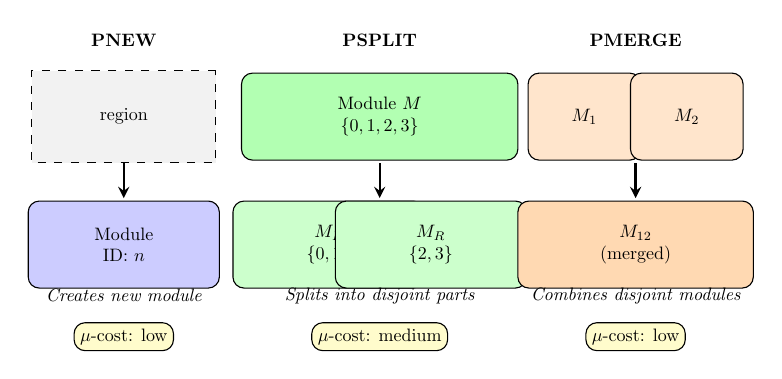
\begin{tikzpicture}[
    module/.style={draw, rounded corners, minimum width=3.2cm, minimum height=1.7cm, align=center, font=\normalsize},
    arrow/.style={->, >=stealth, thick},
    scale=0.65, transform shape
, node distance=3cm]
% PNEW
\node[font=\bfseries] at (-5, 3.5) {PNEW};
\node[draw, dashed, fill=gray!10, minimum width=3.6cm, minimum height=1.8cm] (pnew_before) at (-5, 2) {region};
\draw[arrow, shorten >=2pt, shorten <=2pt] (-5, 1.2) -- (-5, 0.3);
\node[module, fill=blue!20, align=center, text width=3.5cm, font=\normalsize] (pnew_after) at (-5, -0.5) {Module\\ID: $n$};
\node[font=\normalsize\itshape] at (-5, -1.5) {Creates new module};

% PSPLIT
\node[font=\bfseries] at (0, 3.5) {PSPLIT};
\node[module, fill=green!30, minimum width=5.4cm, align=center, text width=3.5cm, font=\normalsize] (psplit_before) at (0, 2) {Module $M$\\$\{0,1,2,3\}$};
\draw[arrow, shorten >=2pt, shorten <=2pt] (0, 1.2) -- (0, 0.3);
\node[module, fill=green!20, minimum width=2.4cm, align=center, text width=3.5cm, font=\normalsize] (psplit_left) at (-1, -0.5) {$M_L$\\$\{0,1\}$};
\node[module, fill=green!20, minimum width=2.4cm, align=center, text width=3.5cm, font=\normalsize] (psplit_right) at (1, -0.5) {$M_R$\\$\{2,3\}$};
\node[font=\normalsize\itshape] at (0, -1.5) {Splits into disjoint parts};

% PMERGE
\node[font=\bfseries] at (5, 3.5) {PMERGE};
\node[module, fill=orange!20, minimum width=2.2cm, font=\normalsize] (pmerge_left) at (4, 2) {$M_1$};
\node[module, fill=orange!20, minimum width=2.2cm, font=\normalsize] (pmerge_right) at (6, 2) {$M_2$};
\draw[arrow, shorten >=2pt, shorten <=2pt] (5, 1.2) -- (5, 0.3);
\node[module, fill=orange!30, minimum width=4.6cm, align=center, text width=3.5cm, font=\normalsize] (pmerge_after) at (5, -0.5) {$M_{12}$\\(merged)};
\node[font=\normalsize\itshape] at (5, -1.5) {Combines disjoint modules};

% Cost annotations
\node[draw, fill=yellow!20, rounded corners, font=\normalsize] at (-5, -2.3) {$\mu$-cost: low};
\node[draw, fill=yellow!20, rounded corners, font=\normalsize] at (0, -2.3) {$\mu$-cost: medium};
\node[draw, fill=yellow!20, rounded corners, font=\normalsize] at (5, -2.3) {$\mu$-cost: low};
\end{tikzpicture}
\caption{The three main partition operations: \texttt{PNEW} creates modules from regions, \texttt{PSPLIT} divides modules into disjoint parts (must cover original), and \texttt{PMERGE} combines disjoint modules. Each operation has an associated $\mu$-cost.}
\label{fig:partition_ops}
\end{figure}

\paragraph{Understanding Figure \ref{fig:partition_ops}:}

\textbf{Three columns (operations):}
\begin{itemize}
    \item \textbf{PNEW (left):} region (dashed box) $\to$ Module ID=$n$ (blue box). Creates new module. $\mu$-cost: low.
    
    \item \textbf{PSPLIT (center):} Module $M$ \{0,1,2,3\} (green) $\to$ $M_L$ \{0,1\} + $M_R$ \{2,3\} (two green boxes). Splits into disjoint parts covering original. $\mu$-cost: medium.
    
    \item \textbf{PMERGE (right):} $M_1$ + $M_2$ (two orange boxes) $\to$ $M_{12}$ (merged, larger orange box). Combines disjoint modules. $\mu$-cost: low.
\end{itemize}

\textbf{Cost annotations (bottom):} Yellow boxes showing relative $\mu$-costs

\textbf{Key insight:} Three ways to modify partition structure. PSPLIT has highest cost (reveals internal structure). PNEW/PMERGE have lower cost (structural bookkeeping).

\textit{Intuition:} Think of \texttt{PNEW} as drawing a circle around a set of memory addresses and saying ``this is now a distinct object.'' If you try to draw a circle around something that is already circled, \texttt{PNEW} simply points to the existing circle, ensuring that you don't pay for the same structure twice.

\subsubsection{PSPLIT: Module Splitting}

\begin{lstlisting}
Definition graph_psplit (g : PartitionGraph) (mid : ModuleID)
  (left right : list nat)
  : option (PartitionGraph * ModuleID * ModuleID) := ...
\end{lstlisting}

\paragraph{Understanding graph\_psplit (Module Splitting):}
\textbf{Function Signature Analysis:}
\begin{itemize}
    \item \textbf{Inputs}: Graph \texttt{g}, module ID to split \texttt{mid}, two sub-regions \texttt{left} and \texttt{right}
    \item \textbf{Output}: \texttt{option} type wrapping a 3-tuple (new graph, left module ID, right module ID)
    \item \textbf{Why option?}: The operation can fail if preconditions aren't met. \texttt{None} = failure, \texttt{Some (...)} = success.
\end{itemize}

\textbf{Precondition Checks (implicit in implementation):}
\begin{enumerate}
    \item \textbf{Partition Property}: \texttt{left $\cup$ right = original\_region} and \texttt{left $\cap$ right = $\emptyset$}
    \begin{itemize}
        \item Every address in the original must appear in exactly one of left/right
        \item No address can appear in both (disjointness)
    \end{itemize}
    \item \textbf{Non-Empty}: Both \texttt{left} and \texttt{right} must contain at least one address
    \item \textbf{Module Exists}: \texttt{mid} must be a valid module in \texttt{g}
\end{enumerate}

\textbf{What Happens on Success:}
\begin{enumerate}
    \item \textbf{Remove Original}: Module \texttt{mid} is removed from the graph
    \item \textbf{Create Two Children}: New modules with regions \texttt{left} and \texttt{right} are added
    \item \textbf{Copy Axioms}: The original module's axiom set is copied to both children (structural information is preserved)
    \item \textbf{Generate Fresh IDs}: Use \texttt{pg\_next\_id} (then increment it twice) to get two new unique IDs
    \item \textbf{Return Tuple}: New graph plus the two new module IDs
\end{enumerate}

\textbf{Information-Theoretic Interpretation:}
\begin{itemize}
    \item \textbf{$\mu$-Cost}: Proportional to $\log_2(\text{number of ways to partition})$. If the original region has $n$ addresses, there are $2^n - 2$ ways to split it (excluding empty partitions).
    \item \textbf{Knowledge Gain}: PSPLIT reveals that the module has internal structure—it's not monolithic but composite.
    \item \textbf{Reversibility}: PSPLIT followed by PMERGE on the two children can recover the original structure, but the $\mu$-cost is not refunded.
\end{itemize}

\texttt{PSPLIT} replaces a module with two sub-modules. Preconditions:
\begin{itemize}
    \item \texttt{left} and \texttt{right} must partition the original region
    \item Neither can be empty
    \item They must be disjoint
\end{itemize}

\textit{Intuition:} Think of \texttt{PSPLIT} as taking a module and slicing it in two. You must prove that the slice is clean (disjoint) and complete (covers the original). This operation allows you to refine your structural view, for example, by realizing that a large array is actually composed of two independent halves.

\subsubsection{PMERGE: Module Merging}

\begin{lstlisting}
Definition graph_pmerge (g : PartitionGraph) (m1 m2 : ModuleID)
  : option (PartitionGraph * ModuleID) := ...
\end{lstlisting}

\paragraph{Understanding graph\_pmerge (Module Merging):}
\textbf{Function Signature:}
\begin{itemize}
    \item \textbf{Inputs}: Graph \texttt{g}, two module IDs \texttt{m1} and \texttt{m2} to merge
    \item \textbf{Output}: \texttt{option} wrapping a pair (new graph, merged module ID)
    \item \textbf{Partial Function}: Returns \texttt{None} if merge preconditions fail
\end{itemize}

\textbf{Precondition Validation:}
\begin{enumerate}
    \item \textbf{Distinct Modules}: $m1 \neq m2$ (cannot merge a module with itself)
    \item \textbf{Both Exist}: Both \texttt{m1} and \texttt{m2} must be valid module IDs in the graph
    \item \textbf{Disjoint Regions}: The two modules' regions must have no overlap: $region_1 \cap region_2 = \emptyset$
    \begin{itemize}
        \item Why? Because modules represent disjoint ownership. Merging overlapping regions would violate the partition property.
    \end{itemize}
\end{enumerate}

\textbf{Merge Operation Steps:}
\begin{enumerate}
    \item \textbf{Union Regions}: \texttt{new\_region = region\_1 $\cup$ region\_2}
    \item \textbf{Concatenate Axioms}: \texttt{new\_axioms = axioms\_1 ++ axioms\_2} (append lists)
    \item \textbf{Remove Both Modules}: Delete \texttt{m1} and \texttt{m2} from the graph
    \item \textbf{Create Merged Module}: Add a new module with \texttt{new\_region} and \texttt{new\_axioms}
    \item \textbf{Generate Fresh ID}: Use (and increment) \texttt{pg\_next\_id}
\end{enumerate}

\textbf{Why Concatenate Axioms?} Because both sets of constraints must hold for the merged module. If module 1 asserts \texttt{x > 0} and module 2 asserts \texttt{y\ is\ prime}, the merged module must satisfy both constraints.

\textbf{$\mu$-Cost Interpretation:}
\begin{itemize}
    \item \textbf{Lower Cost Than Split}: Merging typically costs less than splitting because you're asserting that two things are ``the same kind'' (lower entropy) rather than distinguishing them.
    \item \textbf{Abstraction}: PMERGE is an abstraction operation—forgetting the internal boundary. This can be useful when you want to treat a composite structure as atomic again.
    \item \textbf{Irreversibility}: You cannot recover the original split without additional information. If you merge then split again, you need to re-specify where the boundary was.
\end{itemize}

\textbf{Real-World Analogy:} Think of merging as combining two departments in a company into one. The new department inherits all policies (axioms) from both predecessors, but the organizational boundary is erased.

\texttt{PMERGE} combines two modules into one. Preconditions:
\begin{itemize}
    \item $m1 \neq m2$
    \item The regions must be disjoint
\end{itemize}

Axioms are concatenated in the merged module.

\subsection{Observables and Locality}

\subsubsection{Observable Definition}

An observable extracts what can be seen from outside a module:
\begin{lstlisting}
Definition Observable (s : VMState) (mid : nat) : option (list nat * nat) :=
  match graph_lookup s.(vm_graph) mid with
  | Some modstate => Some (normalize_region modstate.(module_region), s.(vm_mu))
  | None => None
  end.

Definition ObservableRegion (s : VMState) (mid : nat) : option (list nat) :=
  match graph_lookup s.(vm_graph) mid with
  | Some modstate => Some (normalize_region modstate.(module_region))
  | None => None
  end.
\end{lstlisting}

\paragraph{Understanding Observables:}
\textbf{What is an Observable?} In quantum mechanics, an observable is a measurable property. Here, it's the "public interface" of a module—what external code can see without looking inside.

\textbf{Observable Function (Full Version):}
\begin{itemize}
    \item \textbf{Returns Tuple}: (normalized region, global $\mu$-ledger value)
    \item \textbf{Why Include $\mu$?}: Because the $\mu$-ledger is globally observable—all computations can see how much structural cost has been paid.
    \item \textbf{Product Type (*)}: Pairs two values together. Think of it as a struct with two fields.
\end{itemize}

\textbf{ObservableRegion Function (Region Only):}
\begin{itemize}
    \item \textbf{Stripped-Down Version}: Only returns the module's region, not $\mu$
    \item \textbf{Use Case}: When checking locality properties, we only care about region changes
\end{itemize}

\textbf{What's NOT Observable:}
\begin{enumerate}
    \item \textbf{Axioms}: The logical constraints (\texttt{module\_axioms}) are hidden. This is intentional—axioms are \emph{implementation details}.
    \item \textbf{Module Internals}: Cannot see memory contents, only which addresses the module owns
    \item \textbf{Other Modules}: Each observable is isolated to one module
\end{enumerate}

\textbf{Why Normalize?} Two modules with regions \texttt{[1;2;3]} and \texttt{[3;2;1]} should be observationally equivalent. Normalization ensures a canonical form.

\textbf{Option Type Handling:}
\begin{itemize}
    \item \textbf{None}: Module doesn't exist (invalid ID or already removed)
    \item \textbf{Some (...)}: Module exists, return its observable state
\end{itemize}

\textbf{Information Hiding Principle:} Observables define an abstraction barrier. Two states with the same observables are \emph{indistinguishable} to external code, even if their internal axioms differ. This is crucial for locality proofs.

Note that \textbf{axioms are not observable}—they are internal implementation details.

\subsubsection{Observational No-Signaling}

The central locality theorem states that operations on one module cannot affect observables of unrelated modules:

\begin{theorem}[Observational No-Signaling]
If module $\text{mid}$ is not in the target set of instruction $\text{instr}$, then:
\[
\text{ObservableRegion}(s, \text{mid}) = \text{ObservableRegion}(s', \text{mid})
\]
\end{theorem}

Proven as \texttt{observational\_no\_signaling} in the formal development:
\begin{lstlisting}
Theorem observational_no_signaling : forall s s' instr mid,
  well_formed_graph s.(vm_graph) ->
  mid < pg_next_id s.(vm_graph) ->
  vm_step s instr s' ->
  ~ In mid (instr_targets instr) ->
  ObservableRegion s mid = ObservableRegion s' mid.
\end{lstlisting}

\paragraph{Understanding the No-Signaling Theorem:}
\textbf{Theorem Statement Line-by-Line:}
\begin{enumerate}
    \item \textbf{forall s s' instr mid}: For any initial state, final state, instruction, and module ID
    \item \textbf{Premise 1}: \texttt{well\_formed\_graph} — graph satisfies ID discipline invariant
    \item \textbf{Premise 2}: \texttt{mid < pg\_next\_id} — \texttt{mid} is a valid module (exists in graph)
    \item \textbf{Premise 3}: \texttt{vm\_step s instr s'} — there's a valid transition from \texttt{s} to \texttt{s'}
    \item \textbf{Premise 4}: \texttt{$\sim$ In mid (instr\_targets instr)} — \texttt{mid} is NOT in the instruction's target set
    \begin{itemize}
        \item \texttt{$\sim$}: Logical negation ("not")
        \item \texttt{In}: List membership predicate
        \item \texttt{instr\_targets}: Extracts which modules an instruction modifies (e.g., PSPLIT targets one module, PMERGE targets two)
    \end{itemize}
    \item \textbf{Conclusion}: \texttt{ObservableRegion s mid = ObservableRegion s' mid}
    \begin{itemize}
        \item The observable before and after are \emph{identical} (propositional equality)
        \item Not just "similar"—exactly the same Coq value
    \end{itemize}
\end{enumerate}

\textbf{Physical Interpretation (Bell Locality):}
\begin{itemize}
    \item \textbf{No Spooky Action}: Operating on module A cannot instantaneously affect module B's observable state
    \item \textbf{Information Locality}: Information cannot "teleport" between modules without explicit communication
    \item \textbf{Causality}: Effects are local to their causes. No faster-than-light signaling equivalent.
\end{itemize}

\textbf{Why This Matters:}
\begin{enumerate}
    \item \textbf{Compositional Reasoning}: You can reason about module A's behavior without tracking the entire global state
    \item \textbf{Parallel Execution}: Operations on disjoint modules can be parallelized safely
    \item \textbf{Security}: One module cannot covertly observe or interfere with another
    \item \textbf{Debugging}: If a module's behavior changes, the bug must be in operations that target that module
\end{enumerate}

\textbf{Proof Strategy:}
\begin{enumerate}
    \item \textbf{Case Analysis on Instruction}: Pattern match on \texttt{instr} to handle each instruction type
    \item \textbf{Examine instr\_targets}: For each instruction, show what modules it modifies
    \item \textbf{Graph Update Lemmas}: Prove that graph update functions (\texttt{graph\_add\_module}, \texttt{graph\_remove}, etc.) preserve observables of non-target modules
    \item \textbf{Normalization Stability}: Use \texttt{normalize\_region\_idempotent} to show observables remain canonical
\end{enumerate}

\textbf{Contrast with Quantum Mechanics:} In Bell's theorem, quantum entanglement allows correlations that \emph{seem} like signaling but actually aren't (no information transfer). Here, we prove \emph{stronger} isolation—not just no signaling, but complete independence of observables.

This is a computational analog of Bell locality: you cannot signal to a remote module through local operations.

\section{The No Free Insight Theorem}

% =====================================================
% FIGURE: No Free Insight Visualization
% =====================================================
\begin{figure}[ht]
\centering
\begin{tikzpicture}[
    box/.style={draw, rounded corners, minimum width=5.0cm, minimum height=3.2cm, align=center},
    arrow/.style={->, >=stealth, thick},
    scale=0.65, transform shape
, node distance=2cm]
% Before: Large search space
\node[box, fill=red!20, minimum width=8.2cm, minimum height=5.0cm, align=center, text width=3.5cm, font=\normalsize] (omega) at (-5, 0) {
    \textbf{Search Space $\Omega$}\\[0.3cm]
    \large $2^n$ possibilities
};

% After: Reduced search space
\node[box, fill=green!20, minimum width=5.0cm, minimum height=3.2cm, align=center, text width=3.5cm, font=\normalsize] (omega_prime) at (5, 0) {
    \textbf{Reduced $\Omega'$}\\[0.2cm]
    $2^{n-k}$ possibilities
};

% Arrow with cost
\draw[arrow, ultra very thick, blue, shorten >=2pt, shorten <=2pt] (omega) -- (omega_prime) 
    node[pos=0.5, font=\small, above, yshift=6pt] {\textbf{Insight}}
    node[pos=0.5, font=\small, above, yshift=6pt] {Cost: $\Delta\mu \ge k$ bits};

% Conservation equation
\node[draw, fill=yellow!30, rounded corners, font=\normalsize, align=center, text width=3.5cm] at (0, -2.5) {
    \textbf{No Free Insight:}\\[0.2cm]
    $\log|\Omega| - \log|\Omega'| \le \Delta\mu$\\[0.1cm]
    \textit{``Information gained $\le$ cost paid''}
};

% Stronger vs weaker predicates
\node[draw, dashed, fill=blue!10, rounded corners, font=\normalsize, align=center, text width=3.5cm] at (-4, -2.5) {
    Predicate $P_{\text{weak}}$ \\
    \textit{accepts more traces}
};
\node[draw, dashed, fill=green!10, rounded corners, font=\normalsize, align=center, text width=3.5cm] at (4, -2.5) {
    Predicate $P_{\text{strong}}$ \\
    \textit{accepts fewer traces}
};
\draw[arrow, dashed, shorten >=2pt, shorten <=2pt] (-2, -2.5) -- (2, -2.5) node[pos=0.5, font=\small, above, yshift=6pt] {strengthening};
\end{tikzpicture}
\caption{The No Free Insight theorem: reducing the search space (gaining structural insight) requires paying $\mu$-cost. The information-theoretic bound ensures you cannot ``narrow down'' possibilities without expenditure.}
\label{fig:no_free_insight}
\end{figure}

\paragraph{Understanding Figure \ref{fig:no_free_insight}:}

\textbf{Visual:} Similar to Chapter 1's version but in formal theory context.

\textbf{Left:} Large search space $\Omega$ with $2^n$ states

\textbf{Arrow:} Transformation requiring $\Delta\mu$ bits of structural cost

\textbf{Right:} Reduced space $\Omega'$ with $2^{n-k}$ states

\textbf{Conservation law (bottom):} $\Delta\mu \ge \log_2(\Omega) - \log_2(\Omega')$

\textbf{Role in Chapter 3:} Formal statement of the central theorem proven in §3.7. Reducing uncertainty requires paying proportional $\mu$-cost.

\subsection{Receipt Predicates}

A receipt predicate is a function that classifies execution traces:
\begin{lstlisting}
Definition ReceiptPredicate (A : Type) := list A -> bool.
\end{lstlisting}

\paragraph{Understanding Receipt Predicates:}
\textbf{Type Definition Breakdown:}
\begin{itemize}
    \item \textbf{Definition}: Creates a type alias (like typedef)
    \item \textbf{ReceiptPredicate (A : Type)}: Parameterized by type \texttt{A}—the type of receipts
    \item \textbf{:=}: "is defined as"
    \item \textbf{list A -> bool}: A function type that takes a list of \texttt{A} and returns a boolean
\end{itemize}

\textbf{What is a Predicate?} In logic, a predicate is a function that returns true/false, answering "does this satisfy property P?" Here, receipt predicates answer: "does this execution trace satisfy physical constraints?"

\textbf{The Function Type (->):}
\begin{itemize}
    \item \textbf{Input}: \texttt{list A} — a trace of receipts (chronological sequence of measurements/operations)
    \item \textbf{Output}: \texttt{bool} — \texttt{true} = trace is physically realizable, \texttt{false} = violates constraints
\end{itemize}

\textbf{Parameterization by A:} The \texttt{(A : Type)} makes this generic. Could be:
\begin{itemize}
    \item \texttt{ReceiptPredicate CHSHResult} — predicates over CHSH experiment outcomes
    \item \texttt{ReceiptPredicate ThermodynamicEvent} — predicates over entropy measurements
    \item \texttt{ReceiptPredicate Instruction} — predicates over instruction sequences
\end{itemize}

\textbf{Physical Interpretation:} A receipt predicate encodes laws of physics as computational constraints. For example:
\begin{itemize}
    \item \textbf{Classical Physics}: CHSH statistic $S \leq 2$
    \item \textbf{Quantum Physics}: $S \leq 2\sqrt{2}$ (Tsirelson bound)
    \item \textbf{Thermodynamics}: Entropy never decreases
\end{itemize}
These physical laws become \texttt{bool}-valued functions we can prove theorems about.

For example:
\begin{itemize}
    \item \texttt{chsh\_compatible}: All CHSH trials satisfy $S \le 2$ (local realistic)
    \item \texttt{chsh\_quantum}: All trials satisfy $S \le 2\sqrt{2}$ (quantum)
    \item \texttt{chsh\_supra}: Some trial has $S > 2\sqrt{2}$ (supra-quantum)
\end{itemize}

\subsection{Strength Ordering}

Predicate $P_1$ is stronger than $P_2$ if $P_1$ rules out more traces:
\begin{lstlisting}
Definition stronger {A : Type} (P1 P2 : ReceiptPredicate A) : Prop :=
  forall obs, P1 obs = true -> P2 obs = true.
\end{lstlisting}

\paragraph{Understanding Predicate Strength:}
\textbf{Logical Implication:} \texttt{P1} is stronger means it's \emph{more restrictive}. If \texttt{P1} accepts a trace, then \texttt{P2} must also accept it. But \texttt{P2} might accept traces that \texttt{P1} rejects.

\textbf{Mathematical Notation:}
\begin{itemize}
    \item \textbf{\{A : Type\}}: Implicit type parameter—Coq infers \texttt{A} from context
    \item \textbf{forall obs}: For every possible observation trace
    \item \textbf{P1 obs = true -> P2 obs = true}: If \texttt{P1} accepts, then \texttt{P2} accepts
    \item \textbf{Logical Reading}: "\texttt{P1} is a subset of \texttt{P2}" (in terms of accepted traces)
\end{itemize}

\textbf{Example (CHSH):}
\begin{itemize}
    \item \texttt{P\_classical}: Accepts traces with $S \leq 2$ (classical bound)
    \item \texttt{P\_quantum}: Accepts traces with $S \leq 2\sqrt{2}$ (quantum bound)
    \item \textbf{Relationship}: \texttt{P\_classical} is stronger than \texttt{P\_quantum} because:
    \begin{itemize}
        \item If $S \leq 2$, then certainly $S \leq 2\sqrt{2}$ (since $2 < 2\sqrt{2}$)
        \item But $S = 2.5$ satisfies quantum but not classical
    \end{itemize}
\end{itemize}

\textbf{Set-Theoretic Interpretation:} If we think of predicates as sets of traces they accept:
\begin{itemize}
    \item \texttt{stronger P1 P2} means $\{traces \mid P1(trace)\} \subseteq \{traces \mid P2(trace)\}$
    \item Stronger predicate = smaller acceptance set = more constraints
\end{itemize}

Strict strengthening:
\begin{lstlisting}
Definition strictly_stronger {A : Type} (P1 P2 : ReceiptPredicate A) : Prop :=
  (P1 <= P2) /\ (exists obs, P1 obs = false /\ P2 obs = true).
\end{lstlisting}

\paragraph{Understanding Strict Strengthening:}
\textbf{Conjunction ($/\backslash$):} Both conditions must hold:
\begin{enumerate}
    \item \textbf{(P1 <= P2)}: \texttt{P1} is stronger (or equal)
    \item \textbf{exists obs, ...}: There exists at least one trace where they differ
    \begin{itemize}
        \item \texttt{P1 obs = false}: \texttt{P1} rejects this trace
        \item \texttt{P2 obs = true}: But \texttt{P2} accepts it
    \end{itemize}
\end{enumerate}

\textbf{Why "Strictly"?} This rules out the case where \texttt{P1} and \texttt{P2} are equivalent (accept exactly the same traces). We need genuine strengthening—not just a renaming.

\textbf{Witness Requirement:} The \texttt{exists obs} clause requires a constructive witness—an actual trace demonstrating the difference. This isn't abstract—you must exhibit a concrete example.

\textbf{Information-Theoretic Meaning:} Strictly stronger predicates provide more information. Going from \texttt{P2} to \texttt{P1} narrows the possibility space, which costs $\mu$-bits proportional to $\log_2(|P2|/|P1|)$.

\subsection{The Main Theorem}

\begin{theorem}[No Free Insight]
If:
\begin{enumerate}
    \item The system satisfies axioms A1-A4 (non-forgeable receipts, monotone $\mu$, locality, underdetermination)
    \item $P_{\text{strong}} < P_{\text{weak}}$ (strict strengthening)
    \item Execution certifies $P_{\text{strong}}$
\end{enumerate}
Then the trace contains a structure-addition event.
\end{theorem}

Proven as \texttt{strengthening\_requires\_structure\_addition}:
\begin{lstlisting}
Theorem strengthening_requires_structure_addition :
  forall (A : Type)
         (decoder : receipt_decoder A)
         (P_weak P_strong : ReceiptPredicate A)
         (trace : Receipts)
         (s_init : VMState)
         (fuel : nat),
    strictly_stronger P_strong P_weak ->
    s_init.(vm_csrs).(csr_cert_addr) = 0 ->
    Certified (run_vm fuel trace s_init) decoder P_strong trace ->
    has_structure_addition fuel trace s_init.
\end{lstlisting}

\paragraph{Understanding the No Free Insight Theorem:}
\textbf{Theorem Statement Anatomy:}
\begin{itemize}
    \item \textbf{Universal Quantification}: This holds for \emph{any} type \texttt{A}, decoder, predicates, trace, initial state, and fuel
    \item \textbf{Premises (before ->)}:
    \begin{enumerate}
        \item \texttt{strictly\_stronger P\_strong P\_weak}: The strong predicate genuinely narrows possibilities
        \item \texttt{s\_init.(vm\_csrs).(csr\_cert\_addr) = 0}: Start with empty certificate (no prior knowledge)
        \item \texttt{Certified (run\_vm ...) P\_strong trace}: Execution successfully certifies the strong predicate
    \end{enumerate}
    \item \textbf{Conclusion}: \texttt{has\_structure\_addition fuel trace s\_init}
    \begin{itemize}
        \item The trace \emph{must} contain at least one structure-adding operation
        \item Can't achieve strengthening for "free"
    \end{itemize}
\end{itemize}

\textbf{What is \texttt{has\_structure\_addition}?} A predicate that returns true if the trace contains operations like:
\begin{itemize}
    \item \texttt{PSPLIT}: Adds partition boundaries
    \item \texttt{LASSERT}: Adds logical constraints
    \item \texttt{REVEAL}: Explicitly pays for structural information
    \item \texttt{PDISCOVER}: Records discovery evidence
\end{itemize}

\textbf{Physical Interpretation:}
\begin{itemize}
    \item \textbf{No Perpetual Motion}: Can't extract information (narrow predicates) without paying thermodynamic/computational cost
    \item \textbf{Conservation Law}: Information gain $\leftrightarrow$ structure addition $\leftrightarrow$ $\mu$-cost increase
    \item \textbf{Landauer's Principle Connection}: Structure addition corresponds to bit erasure/commitment, which has minimum energy cost $k_B T \ln 2$
\end{itemize}

\textbf{Why This Matters:}
\begin{enumerate}
    \item \textbf{Falsifiability}: If someone claims to solve NP-complete problems efficiently, check their $\mu$-ledger. It must grow.
    \item \textbf{Quantum Advantage Bound}: Achieving quantum correlations costs structural $\mu$-bits. Can't be "free."
    \item \textbf{Machine Learning}: Training a model (strengthening predictions) requires data, which costs information-theoretically.
\end{enumerate}

\textbf{Proof Strategy:}
\begin{enumerate}
    \item \textbf{Contradiction}: Assume no structure addition
    \item \textbf{Show}: Then partition graph unchanged, axioms unchanged
    \item \textbf{Conclude}: Observables unchanged $\rightarrow$ can't certify stronger predicate
    \item \textbf{Contradiction}: But premise says we did certify it!
\end{enumerate}

\subsection{Revelation Requirement}

As a corollary, I prove that supra-quantum certification requires explicit revelation:

\begin{lstlisting}
Theorem nonlocal_correlation_requires_revelation :
  forall (trace : Trace) (s_init s_final : VMState) (fuel : nat),
    trace_run fuel trace s_init = Some s_final ->
    s_init.(vm_csrs).(csr_cert_addr) = 0 ->
    has_supra_cert s_final ->
    uses_revelation trace \/
    (exists n m p mu, nth_error trace n = Some (instr_emit m p mu)) \/
    (exists n c1 c2 mu, nth_error trace n = Some (instr_ljoin c1 c2 mu)) \/
    (exists n m f c mu, nth_error trace n = Some (instr_lassert m f c mu)).
\end{lstlisting}

\paragraph{Understanding the Revelation Requirement:}
\textbf{Theorem Structure:}
\begin{itemize}
    \item \textbf{Premises}:
    \begin{enumerate}
        \item \texttt{trace\_run ... = Some s\_final}: Execution succeeded (not stuck)
        \item \texttt{csr\_cert\_addr = 0}: Started with no certificate
        \item \texttt{has\_supra\_cert s\_final}: Final state contains supra-quantum certificate (CHSH $S > 2\sqrt{2}$)
    \end{enumerate}
    \item \textbf{Conclusion (Disjunction \\/):} At least ONE of these must be true:
    \begin{enumerate}
        \item \texttt{uses\_revelation trace}: Trace contains explicit REVEAL instruction
        \item \texttt{(exists ... instr\_emit ...)}: Contains EMIT (information output)
        \item \texttt{(exists ... instr\_ljoin ...)}: Contains LJOIN (certificate composition)
        \item \texttt{(exists ... instr\_lassert ...)}: Contains LASSERT (axiom assertion)
    \end{enumerate}
\end{itemize}

\textbf{The \texttt{exists} Pattern:}
\begin{itemize}
    \item \textbf{exists n m p mu}: There exist values \texttt{n}, \texttt{m}, \texttt{p}, \texttt{mu} such that...
    \item \textbf{nth\_error trace n = Some (...)}: The \texttt{n}-th instruction in the trace is this specific instruction
    \item \textbf{Constructive Proof}: Must exhibit actual indices and instruction parameters
\end{itemize}

\textbf{Physical Meaning:}
\begin{itemize}
    \item \textbf{Supra-Quantum Correlations Are Not Free}: Cannot passively observe $S > 2\sqrt{2}$ without active structural operations
    \item \textbf{No Hidden Variables Loophole}: The theorem closes the loophole where someone might claim "the structure was always there, we just measured it"
    \item \textbf{Explicit Cost}: Must use instructions that explicitly charge $\mu$-cost
\end{itemize}

\textbf{Why Disjunction?} Different paths to supra-quantum certification:
\begin{itemize}
    \item \textbf{REVEAL}: Pay direct cost to expose hidden structure
    \item \textbf{EMIT}: Output information (equivalent to revealing)
    \item \textbf{LJOIN}: Combine certificates (requires prior structure addition)
    \item \textbf{LASSERT}: Assert logical constraints (adds axiom structure)
\end{itemize}

\textbf{Falsification Criterion:} If someone claims: "I achieved supra-quantum correlations without paying computational cost," inspect their trace. This theorem guarantees you'll find at least one high-cost instruction. If not, the claim is provably false.

This proves that you cannot achieve "free" quantum advantage—the structural cost must be paid explicitly.

\section{Gauge Symmetry and Conservation}

\subsection{$\mu$-Gauge Transformation}

A gauge transformation shifts the $\mu$-ledger by a constant:
\begin{lstlisting}
Definition mu_gauge_shift (k : nat) (s : VMState) : VMState :=
  {| vm_regs := s.(vm_regs);
     vm_mem := s.(vm_mem);
     vm_csrs := s.(vm_csrs);
     vm_pc := s.(vm_pc);
     vm_graph := s.(vm_graph);
     vm_mu := s.(vm_mu) + k;
     vm_err := s.(vm_err) |}.
\end{lstlisting}

\paragraph{Understanding Gauge Transformations:}
\textbf{What is a Gauge Transformation?} In physics, a gauge transformation is a change in description that doesn't affect physical observables. Like changing coordinates: the physics stays the same.

\textbf{Record Construction Syntax:}
\begin{itemize}
    \item \textbf{\{| ... |\}}: Constructs a new VMState record
    \item \textbf{field := value}: Sets each field explicitly
    \item \textbf{Most Fields Unchanged}: Copies directly from input state \texttt{s}
    \item \textbf{Exception}: \texttt{vm\_mu := s.(vm\_mu) + k} — only the $\mu$-ledger shifts
\end{itemize}

\textbf{Gauge Shift Intuition:}
\begin{itemize}
    \item \textbf{Absolute vs. Relative}: The absolute value of $\mu$ is arbitrary (like choosing origin on a number line)
    \item \textbf{What Matters}: Differences in $\mu$ between states (relative costs)
    \item \textbf{Analogy}: Like setting a timer—whether it shows 0:00 or 1:00 at start doesn't matter, only elapsed time counts
\end{itemize}

\textbf{Why k : nat?} The shift amount is a natural number. Always non-negative—we never shift backward (that would violate monotonicity).

\textbf{Invariants Under Gauge Shift:}
\begin{itemize}
    \item \textbf{Partition Graph}: Unchanged
    \item \textbf{Memory}: Unchanged
    \item \textbf{Registers}: Unchanged
    \item \textbf{Program Counter}: Unchanged
\end{itemize}
Only the "zero point" of the $\mu$-ledger moves.

\subsection{Gauge Invariance}

Partition structure is gauge-invariant:
\begin{lstlisting}
Theorem kernel_conservation_mu_gauge : forall s k,
  conserved_partition_structure s = 
  conserved_partition_structure (nat_action k s).
\end{lstlisting}

\paragraph{Understanding Gauge Invariance:}
\textbf{Theorem Statement:}
\begin{itemize}
    \item \textbf{forall s k}: For any state and any shift amount
    \item \textbf{conserved\_partition\_structure}: A function extracting the partition graph structure (ignoring $\mu$ value)
    \item \textbf{nat\_action k s}: Applies the gauge shift by \texttt{k} to state \texttt{s}
    \item \textbf{Equality}: The extracted structure is identical before and after
\end{itemize}

\textbf{What This Proves:}
\begin{enumerate}
    \item \textbf{Structural Independence}: Partition structure doesn't depend on absolute $\mu$ value
    \item \textbf{Only Deltas Matter}: Instructions cost relative $\mu$-amounts, not absolute levels
    \item \textbf{Gauge Freedom}: Can choose any "zero point" for $\mu$ without changing semantics
\end{enumerate}

\textbf{Noether's Theorem Connection:} In physics, Noether's theorem states:
\[
\text{Symmetry} \leftrightarrow \text{Conservation Law}
\]
Here:
\begin{itemize}
    \item \textbf{Symmetry}: Gauge freedom (can shift $\mu$ arbitrarily)
    \item \textbf{Conservation Law}: Partition structure is conserved (doesn't change under shift)
\end{itemize}

\textbf{Practical Implication:} When verifying 3-way isomorphism (Coq, Python, Verilog), we only need to check that $\mu$ \emph{changes} match, not absolute values. If implementation A starts at $\mu=0$ and B starts at $\mu=1000$, that's fine—just verify increments are identical.

\textbf{Proof Strategy:}
\begin{itemize}
    \item \textbf{Unfold Definitions}: Expand \texttt{conserved\_partition\_structure} and \texttt{nat\_action}
    \item \textbf{Simplify}: Show that partition graph field is unchanged by gauge shift
    \item \textbf{Reflexivity}: Both sides reduce to \texttt{s.(vm\_graph)}
\end{itemize}

This is the computational analog of Noether's theorem: the gauge symmetry (ability to shift $\mu$ by a constant) corresponds to the conservation of partition structure.

% =====================================================
% FIGURE: Gauge Symmetry
% =====================================================
\begin{figure}[ht]
\centering
\begin{tikzpicture}[scale=1.8, 
    state/.style={draw, rounded corners, minimum width=5.4cm, minimum height=4.6cm, align=center},
    arrow/.style={->, >=stealth, thick}
, node distance=2cm]
% Original state
\node[state, fill=blue!15, align=center, text width=3.5cm, font=\normalsize] (s) at (-3, 0) {
    \textbf{State $s$}\\[0.2cm]
    $\mu = \mu_0$\\
    $\Pi = \Pi_0$
};

% Shifted state
\node[state, fill=blue!15, align=center, text width=3.5cm, font=\normalsize] (sk) at (3, 0) {
    \textbf{State $s + k$}\\[0.2cm]
    $\mu = \mu_0 + k$\\
    $\Pi = \Pi_0$
};

% Gauge transformation arrow
\draw[arrow, ultra very thick, purple, shorten >=2pt, shorten <=2pt] (s) -- (sk) 
    node[pos=0.5, font=\small, above, yshift=6pt] {Gauge Shift $+k$};

% Invariant annotation
\node[draw, fill=yellow!20, rounded corners, font=\normalsize, align=center, text width=3.5cm] at (0, -2) {
    \textbf{Gauge Invariant:}\\
    Partition structure $\Pi$ unchanged\\[0.1cm]
    \textit{(Computational Noether's Theorem)}
};

% Physical analogy
\node[draw, dashed, fill=green!10, rounded corners, font=\normalsize, align=center, text width=3.5cm] at (0, -3.5) {
    \textbf{Physical Analog:}\\
    Energy zero-point is arbitrary\\
    Only \textit{differences} matter
};
\end{tikzpicture}
\caption{Gauge symmetry: shifting the $\mu$-ledger by a constant $k$ leaves the partition structure invariant. This is the computational analog of Noether's theorem---the gauge symmetry corresponds to conservation of structural decomposition.}
\label{fig:gauge_symmetry}
\end{figure}

\paragraph{Understanding Figure \ref{fig:gauge_symmetry}:}

\textbf{Transformation:} $\mu \mapsto \mu + k$ (shift by constant)

\textbf{Two views:} States $(s, \mu)$ and $(s, \mu+k)$ are shown to be structurally equivalent

\textbf{Key property:} Partition graph $\Pi$ is invariant under shift - structure unchanged

\textbf{Physical analogy:} Like gauge symmetry in physics. Shifting the potential by a constant doesn't change the physics (only differences matter).

\textbf{Computational analog:} Absolute $\mu$ value is gauge-dependent. Only $\mu$ differences (costs) are physically meaningful.

\textbf{Noether's theorem connection:} Gauge symmetry $\leftrightarrow$ Conservation law. Here: $\mu$-shift symmetry $\leftrightarrow$ Partition structure conservation.

\section{Chapter Summary}

% =====================================================
% FIGURE: Chapter 3 Summary
% =====================================================
\begin{figure}[ht]
\centering
\begin{tikzpicture}[
    concept/.style={draw, rounded corners, minimum width=4.0cm, minimum height=2.4cm, align=center, font=\normalsize},
    result/.style={draw, very thick, fill=yellow!20, rounded corners, minimum width=6.2cm, minimum height=1.7cm, align=center, font=\normalsize},
    scale=0.65, transform shape
, node distance=2.5cm]
% Core concepts
\node[concept, fill=blue!20, align=center, text width=3.5cm] (state) at (-4, 3) {State Space\\$S$};
\node[concept, fill=green!20, align=center, text width=3.5cm] (partition) at (-1.5, 3) {Partition Graph\\$\Pi$};
\node[concept, fill=orange!20, align=center, text width=3.5cm] (mu) at (1.5, 3) {$\mu$-Ledger\\Currency};
\node[concept, fill=red!20, align=center, text width=3.5cm] (rules) at (4, 3) {Transition\\Rules $R$};

% Key theorems
\node[result, align=center, text width=3.5cm] (mono) at (-2.5, 0.5) {\textbf{$\mu$-Monotonicity}\\$s'.\mu \ge s.\mu$};
\node[result, align=center, text width=3.5cm] (nosig) at (2.5, 0.5) {\textbf{No-Signaling}\\Local ops $\not\to$ remote observables};

% Master result
\node[draw, ultra very thick, fill=green!30, rounded corners, minimum width=14.4cm, minimum height=2.6cm, align=center, text width=3.5cm] (master) at (0, -2) {
    \textbf{No Free Insight Theorem}\\
    $\log|\Omega| - \log|\Omega'| \le \Delta\mu$
};

% Arrows
\draw[->, very thick, shorten >=2pt, shorten <=2pt] (state) -- (mono);
\draw[->, very thick, shorten >=2pt, shorten <=2pt] (partition) -- (mono);
\draw[->, very thick, shorten >=2pt, shorten <=2pt] (partition) -- (nosig);
\draw[->, very thick, shorten >=2pt, shorten <=2pt] (rules) -- (nosig);
\draw[->, very thick, shorten >=2pt, shorten <=2pt] (mu) -- (mono);
\draw[->, very thick, shorten >=2pt, shorten <=2pt] (mono) -- (master);
\draw[->, very thick, shorten >=2pt, shorten <=2pt] (nosig) -- (master);

% Chapter reference
\node[ below=0.5cm of master, font=\small, yshift=-6pt] {Foundation for Chapters 4 (Implementation), 5 (Verification), and 6 (Tsirelson)};
\end{tikzpicture}
\caption{Chapter 3 summary: The formal model $(S, \Pi, A, R, L)$ leads to two key properties ($\mu$-monotonicity and no-signaling), which together establish the No Free Insight theorem---the theoretical foundation for the Tsirelson bound derivation.}
\label{fig:ch3_summary}
\end{figure}

\paragraph{Understanding Figure \ref{fig:ch3_summary}:}

\textbf{Top:} Formal model $(S, \Pi, A, R, L)$ - the five components defined in this chapter

\textbf{Middle (two branches):}
\begin{itemize}
    \item Left: $\mu$-monotonicity - ledger never decreases
    \item Right: No-signaling - locality enforcement
\end{itemize}

\textbf{Bottom:} No Free Insight theorem - the convergence of both properties

\textbf{Final arrow:} Points to Tsirelson bound derivation (next chapter)

\textbf{Key insight:} This chapter builds the formal foundation. The model's two key properties ($\mu$-monotonicity + locality) combine to prove No Free Insight, which leads to the Tsirelson bound $2\sqrt{2}$ in Chapter 4.

This chapter has defined the Thiele Machine as a formal 5-tuple $T = (S, \Pi, A, R, L)$ with the following key results:

\begin{enumerate}
    \item \textbf{State Space} ($S$): A structured record with explicit partition graph, registers, memory, and the $\mu$-ledger.
    
    \item \textbf{Partition Graph} ($\Pi$): Modules decompose state into disjoint regions with monotonic ID assignment and well-formedness invariants.
    
    \item \textbf{$\mu$-bit Currency}: A monotonic counter that bounds structural information cost. The ledger satisfies:
    \begin{itemize}
        \item Single-step monotonicity: $s'.\mu \ge s.\mu$
        \item Multi-step conservation: $\mu_n = \mu_0 + \sum \text{cost}(op_i)$
        \item Irreversibility bound: connects to Landauer's principle
    \end{itemize}
    
    \item \textbf{No-Signaling}: Local operations cannot affect observables of non-target modules.
    
    \item \textbf{No Free Insight}: Any strengthening of receipt predicates requires structure-addition events (and thus $\mu$-cost).
    
    \item \textbf{Gauge Symmetry}: The partition structure is invariant under $\mu$-shifts (computational Noether's theorem).
\end{enumerate}

These formal foundations enable the implementation (Chapter 4), verification (Chapter 5), and the derivation of the Tsirelson bound from pure $\mu$-accounting (Chapter 6).
